\documentclass[UTF8,11pt,a4paper,oneside,fontset=none]{ctexart}

\usepackage[a4paper,top=1.8cm,bottom=1.8cm,left=1.9cm,right=1.9cm,headheight=15pt]{geometry}
\usepackage{fontspec}
\usepackage{amsmath,amssymb,mathtools,bm}
\usepackage{unicode-math}
\usepackage{booktabs,tabularx,array,multirow,longtable}
\usepackage[table]{xcolor}
\usepackage{graphicx,float}
\usepackage{siunitx}
\usepackage{enumitem}
\usepackage{fancyhdr}
\usepackage{caption}
\usepackage{hyperref}
\usepackage[most]{tcolorbox}
\usepackage{pdflscape}

\setmainfont{Times New Roman}
\setsansfont{Arial}
\setmonofont{Consolas}
\setmathfont{Cambria Math}
\setCJKmainfont[BoldFont=SimHei,ItalicFont=KaiTi]{SimSun}
\setCJKsansfont[BoldFont={Microsoft YaHei Bold}]{Microsoft YaHei}
\setCJKmonofont{FangSong}

\definecolor{DeepBlue}{HTML}{17324D}
\definecolor{PandaTeal}{HTML}{0B7A75}
\definecolor{WarmGold}{HTML}{C58A19}
\definecolor{Coral}{HTML}{C95F4A}
\definecolor{SoftBlue}{HTML}{EEF5F8}
\definecolor{SoftTeal}{HTML}{ECF7F5}
\definecolor{SoftGold}{HTML}{FFF7E7}
\definecolor{SoftRed}{HTML}{FFF0F0}
\definecolor{MidGray}{HTML}{667085}
\definecolor{LineGray}{HTML}{D5DEE5}
\definecolor{PassGreen}{HTML}{237A45}

\hypersetup{
  colorlinks=true,
  linkcolor=DeepBlue,
  urlcolor=PandaTeal,
  pdfauthor={范子恒},
  pdftitle={PandaX-4T 独立能量重建完整报告}
}
\ctexset{
  section={format=\Large\bfseries\color{DeepBlue},number=\arabic{section},
    beforeskip=0.8em,afterskip=0.7em},
  subsection={format=\large\bfseries\color{PandaTeal}},
  subsubsection={format=\normalsize\bfseries\color{DeepBlue}}
}

\pagestyle{fancy}
\fancyhf{}
\fancyhead[L]{\small\color{DeepBlue}PandaX-4T 能量重建}
\fancyhead[R]{\small\color{MidGray}完整技术报告 · candidate\_v11}
\fancyfoot[C]{\small\color{MidGray}\thepage}
\renewcommand{\headrulewidth}{0.4pt}
\renewcommand{\footrulewidth}{0pt}

\captionsetup{font=small,labelfont=bf,labelsep=quad}
\graphicspath{{figures/}}
\setlength{\parindent}{2em}
\setlength{\parskip}{0.24em}
\setlist[itemize]{leftmargin=1.8em,itemsep=0.28em,topsep=0.3em}
\setlist[enumerate]{leftmargin=2em,itemsep=0.3em,topsep=0.3em}
\renewcommand{\arraystretch}{1.18}
\sisetup{group-separator={,},group-minimum-digits=4}

\newcolumntype{Y}{>{\raggedright\arraybackslash}X}
\newcolumntype{C}[1]{>{\centering\arraybackslash}p{#1}}
\newcolumntype{R}[1]{>{\raggedleft\arraybackslash}p{#1}}
\newcommand{\var}[1]{\texttt{\detokenize{#1}}}
\newcommand{\pass}{\textcolor{PassGreen}{\textbf{PASS}}}
\newcommand{\pending}{\textcolor{WarmGold}{\textbf{待验证}}}
\newcommand{\Rfit}{R_{\mathrm{fit}}}
\newcommand{\Rsixtyeight}{R_{68}}
\newcommand{\Rninty}{R_{90}}

\newtcolorbox{infobox}[1][]{enhanced,breakable,colback=SoftBlue,colframe=DeepBlue,
  boxrule=0.7pt,arc=1.7mm,left=1.6mm,right=1.6mm,top=1.2mm,bottom=1.2mm,#1}
\newtcolorbox{scopebox}[1][]{enhanced,breakable,colback=SoftRed,colframe=Coral,
  boxrule=0.75pt,arc=1.7mm,title={结论边界},fonttitle=\bfseries,
  left=1.6mm,right=1.6mm,top=1.2mm,bottom=1.2mm,#1}
\newtcolorbox{notebox}[1][]{enhanced,breakable,colback=SoftGold,colframe=WarmGold,
  boxrule=0.75pt,arc=1.7mm,title={理解提示},fonttitle=\bfseries,
  left=1.6mm,right=1.6mm,top=1.2mm,bottom=1.2mm,#1}
\newtcolorbox{conclusionbox}[1][]{enhanced,breakable,colback=SoftTeal,colframe=PandaTeal,
  boxrule=0.85pt,arc=1.7mm,title={本节结论},fonttitle=\bfseries,
  left=1.6mm,right=1.6mm,top=1.2mm,bottom=1.2mm,#1}

\begin{document}

\begin{titlepage}
\thispagestyle{empty}
\vspace*{0.7cm}
\noindent{\color{PandaTeal}\rule{\textwidth}{3.8pt}}
\vspace{1.0cm}

{\sffamily\bfseries\fontsize{25pt}{32pt}\selectfont\color{DeepBlue}
PandaX-4T 独立能量重建\par 完整技术报告\par}
\vspace{0.38cm}
{\sffamily\bfseries\fontsize{15pt}{22pt}\selectfont\color{PandaTeal}
从原始标量数据、验证设计到强化模型 candidate\_v11\par}

\vspace{0.9cm}
\begin{tcolorbox}[colback=SoftBlue,colframe=DeepBlue,boxrule=0.9pt,arc=2mm,
  left=3mm,right=3mm,top=2.5mm,bottom=2.5mm]
\centering
{\sffamily\bfseries\large 报告目标}\par\vspace{1mm}
不依赖已有重建工作的模型参数，从 Run 10972 的标量数据和变量定义出发，\par
建立可复核、可冻结、可由老师在新数据上独立运行的能量修正流程。\par
\end{tcolorbox}

\vspace{0.65cm}
\begin{center}
\begin{tabular}{C{4.7cm} C{4.7cm} C{4.7cm}}
\begin{tcolorbox}[width=4.45cm,colback=white,colframe=LineGray,arc=1.5mm,halign=center]
{\sffamily\bfseries\fontsize{21pt}{24pt}\selectfont\color{DeepBlue}4499}\par
\small 有效事件
\end{tcolorbox}
&
\begin{tcolorbox}[width=4.45cm,colback=white,colframe=LineGray,arc=1.5mm,halign=center]
{\sffamily\bfseries\fontsize{21pt}{24pt}\selectfont\color{PandaTeal}64}\par
\small 受控输入变量
\end{tcolorbox}
&
\begin{tcolorbox}[width=4.45cm,colback=white,colframe=LineGray,arc=1.5mm,halign=center]
{\sffamily\bfseries\fontsize{21pt}{24pt}\selectfont\color{WarmGold}0.9973\%}\par
\small 合并 OOF \(\sigma/\mu\)
\end{tcolorbox}
\end{tabular}
\end{center}

\vspace{0.35cm}
\begin{scopebox}
本报告中的主结果来自 Run 10972 内按完整采集文件块形成的未见预测。
它不是独立新 run 的最终结论，也不应被表述为 PandaX-4T 的最终物理能量分辨率。
\end{scopebox}

\vfill
\noindent\begin{tabularx}{\textwidth}{@{}Y R{5.5cm}@{}}
\textbf{报告人：}范子恒 & \textbf{数据：}Run 10972\\
\textbf{当前模型：}candidate\_v11 & \textbf{日期：}2026 年 7 月 31 日
\end{tabularx}
\vspace{0.25cm}
\end{titlepage}

\pagenumbering{Roman}
\section*{摘要}
\addcontentsline{toc}{section}{摘要}

本项目研究 PandaX-4T 标定数据中 \(\SI{2614.5}{keV}\) 单能峰的能量重建。
与具有逐事件真实标签的普通回归不同，这里的监督信息主要来自“整批事件应围绕同一峰中心”。
因此，目标不是拟合某个给定的逐事件答案，而是在严格隔离的未见采集文件块上减小
\(\sigma/\mu\)，同时控制峰中心、尾部、修正幅度和数值安全。

我们从上游标量 TXT 出发，检查 4500 行、188 个字段及 985 个
\var{fileNumber} 的覆盖；使用 \var{qS1ub_C} 与 \var{qS2Bdesub_C}
构造基础能量方向；比较当前线性公式、已有三次多项式
\var{Energy_cor}、训练侧选择的 image foundation 和新模型 candidate\_v11。
模型先在训练侧比较多条 S1/S2 基础信号路径，再以三次样条表达平滑环境响应，
以 Ridge 限制容量，并用
\(0.10\tanh(\cdot/0.10)\) 限制单事件对数修正。

基础路径、变量层级和正则强度均在外层训练池内部选择。
最终冻结方案使用 64 个位置、漂移、脉冲形状、PMT 图样和事件环境变量。
合并 OOF 的 \(\Rfit\) 从当前线性公式的 \(4.1696\%\) 和已有三次式的
\(4.1847\%\) 降至 \(0.9973\%\)；五个外层文件块均低于 \(1.00\%\)。
\(\Rsixtyeight\) 降至 \(1.3674\%\)，
\(\Rninty\) 降至 \(4.2483\%\)。
目前最重要的限制是尚未获得独立新 run，且峰形拟合优度仍不理想。

\begin{infobox}
\textbf{一句话结论：}
我们已经完成了一个内部文件块验证显著优于 v10、可以交给老师盲测的候选模型；
但它仍是 candidate，而不是已经由独立数据证明的最终模型。
\end{infobox}

\clearpage
\tableofcontents
\clearpage
\pagenumbering{arabic}

\section{研究背景：我们究竟在重建什么}

\subsection{双相液氙探测器中的 S1 与 S2}

粒子在液氙中沉积能量后，会产生激发和电离。激发形成初级闪烁光信号 S1；
未复合电子在电场中漂移到液面，经气相放大形成 S2。两者对同一次能量沉积提供互补信息：
复合增强时 S1 往往增加而 S2 减少，因此二者具有反相关结构。

漂移时间 \(dt\) 近似反映纵向位置；S2 光型重建得到的 \(x,y\) 反映横向位置。
光收集效率、电子寿命、PMT 图样、脉冲宽度和事件环境都会使相同真实能量产生略有不同的观测量。
能量重建的工作，就是在不过度拟合的前提下消除这些探测器响应差异。

\subsection{为什么目标是 \texorpdfstring{\(\sigma/\mu\)}{sigma/mu}}

对于理想单能峰，重建能量集中在峰中心 \(\mu\) 附近，其高斯核心宽度为 \(\sigma\)。
相对能量分辨率定义为
\begin{equation}
R=\frac{\sigma}{\mu}.
\end{equation}
\(R\) 越小，说明相同能量事件重建得越集中。但如果模型只是把事件强行压向一个常数，
也会得到很小的峰宽。因此必须同时检查：
\begin{itemize}
  \item 峰中心是否仍接近 \(\SI{2614.5}{keV}\)；
  \item 输出是否有限且为正；
  \item 修正是否大量触及上限；
  \item S1、S2 的基本单调响应是否被破坏；
  \item 尾部宽度和不同采集文件块是否共同改善。
\end{itemize}

\begin{notebox}
本任务没有可靠的逐事件真实能量标签。模型学习的是“哪些探测器状态会使同一单能峰事件偏高或偏低”，
而不是学习某个外部提供的逐事件答案。
\end{notebox}

\section{数据来源、结构与使用边界}

\subsection{输入数据的准确含义}

输入文件为 \var{light_ana_run10972_finalSS_Egt2MeV_scalar.txt}。
这里的“原始数据”指本项目直接收到的上游标量表，不是未经处理的原始波形。
文件名中的 \var{finalSS} 和 \var{Egt2MeV} 表明数据可能已经经过单散射和能量阈值选择。

\begin{table}[H]
\centering
\caption{输入数据概况}
\begin{tabularx}{0.92\textwidth}{lY}
\toprule
项目 & 内容\\
\midrule
Run & 10972\\
输入行数 & 4500\\
有效建模事件 & 4499；1 行基础 S1/S2 不满足有限正值条件\\
字段数 & 188\\
采集文件身份 & 985 个不同的 \var{fileNumber}\\
主要基础信号 & \var{qS1ub_C}、\var{qS2Bdesub_C}\\
位置与环境 & \(dt\)、多套 \(x,y\)、宽度、PMT 图样、预峰活动等\\
\bottomrule
\end{tabularx}
\end{table}

\subsection{基础分布}

\begin{figure}[H]
\centering
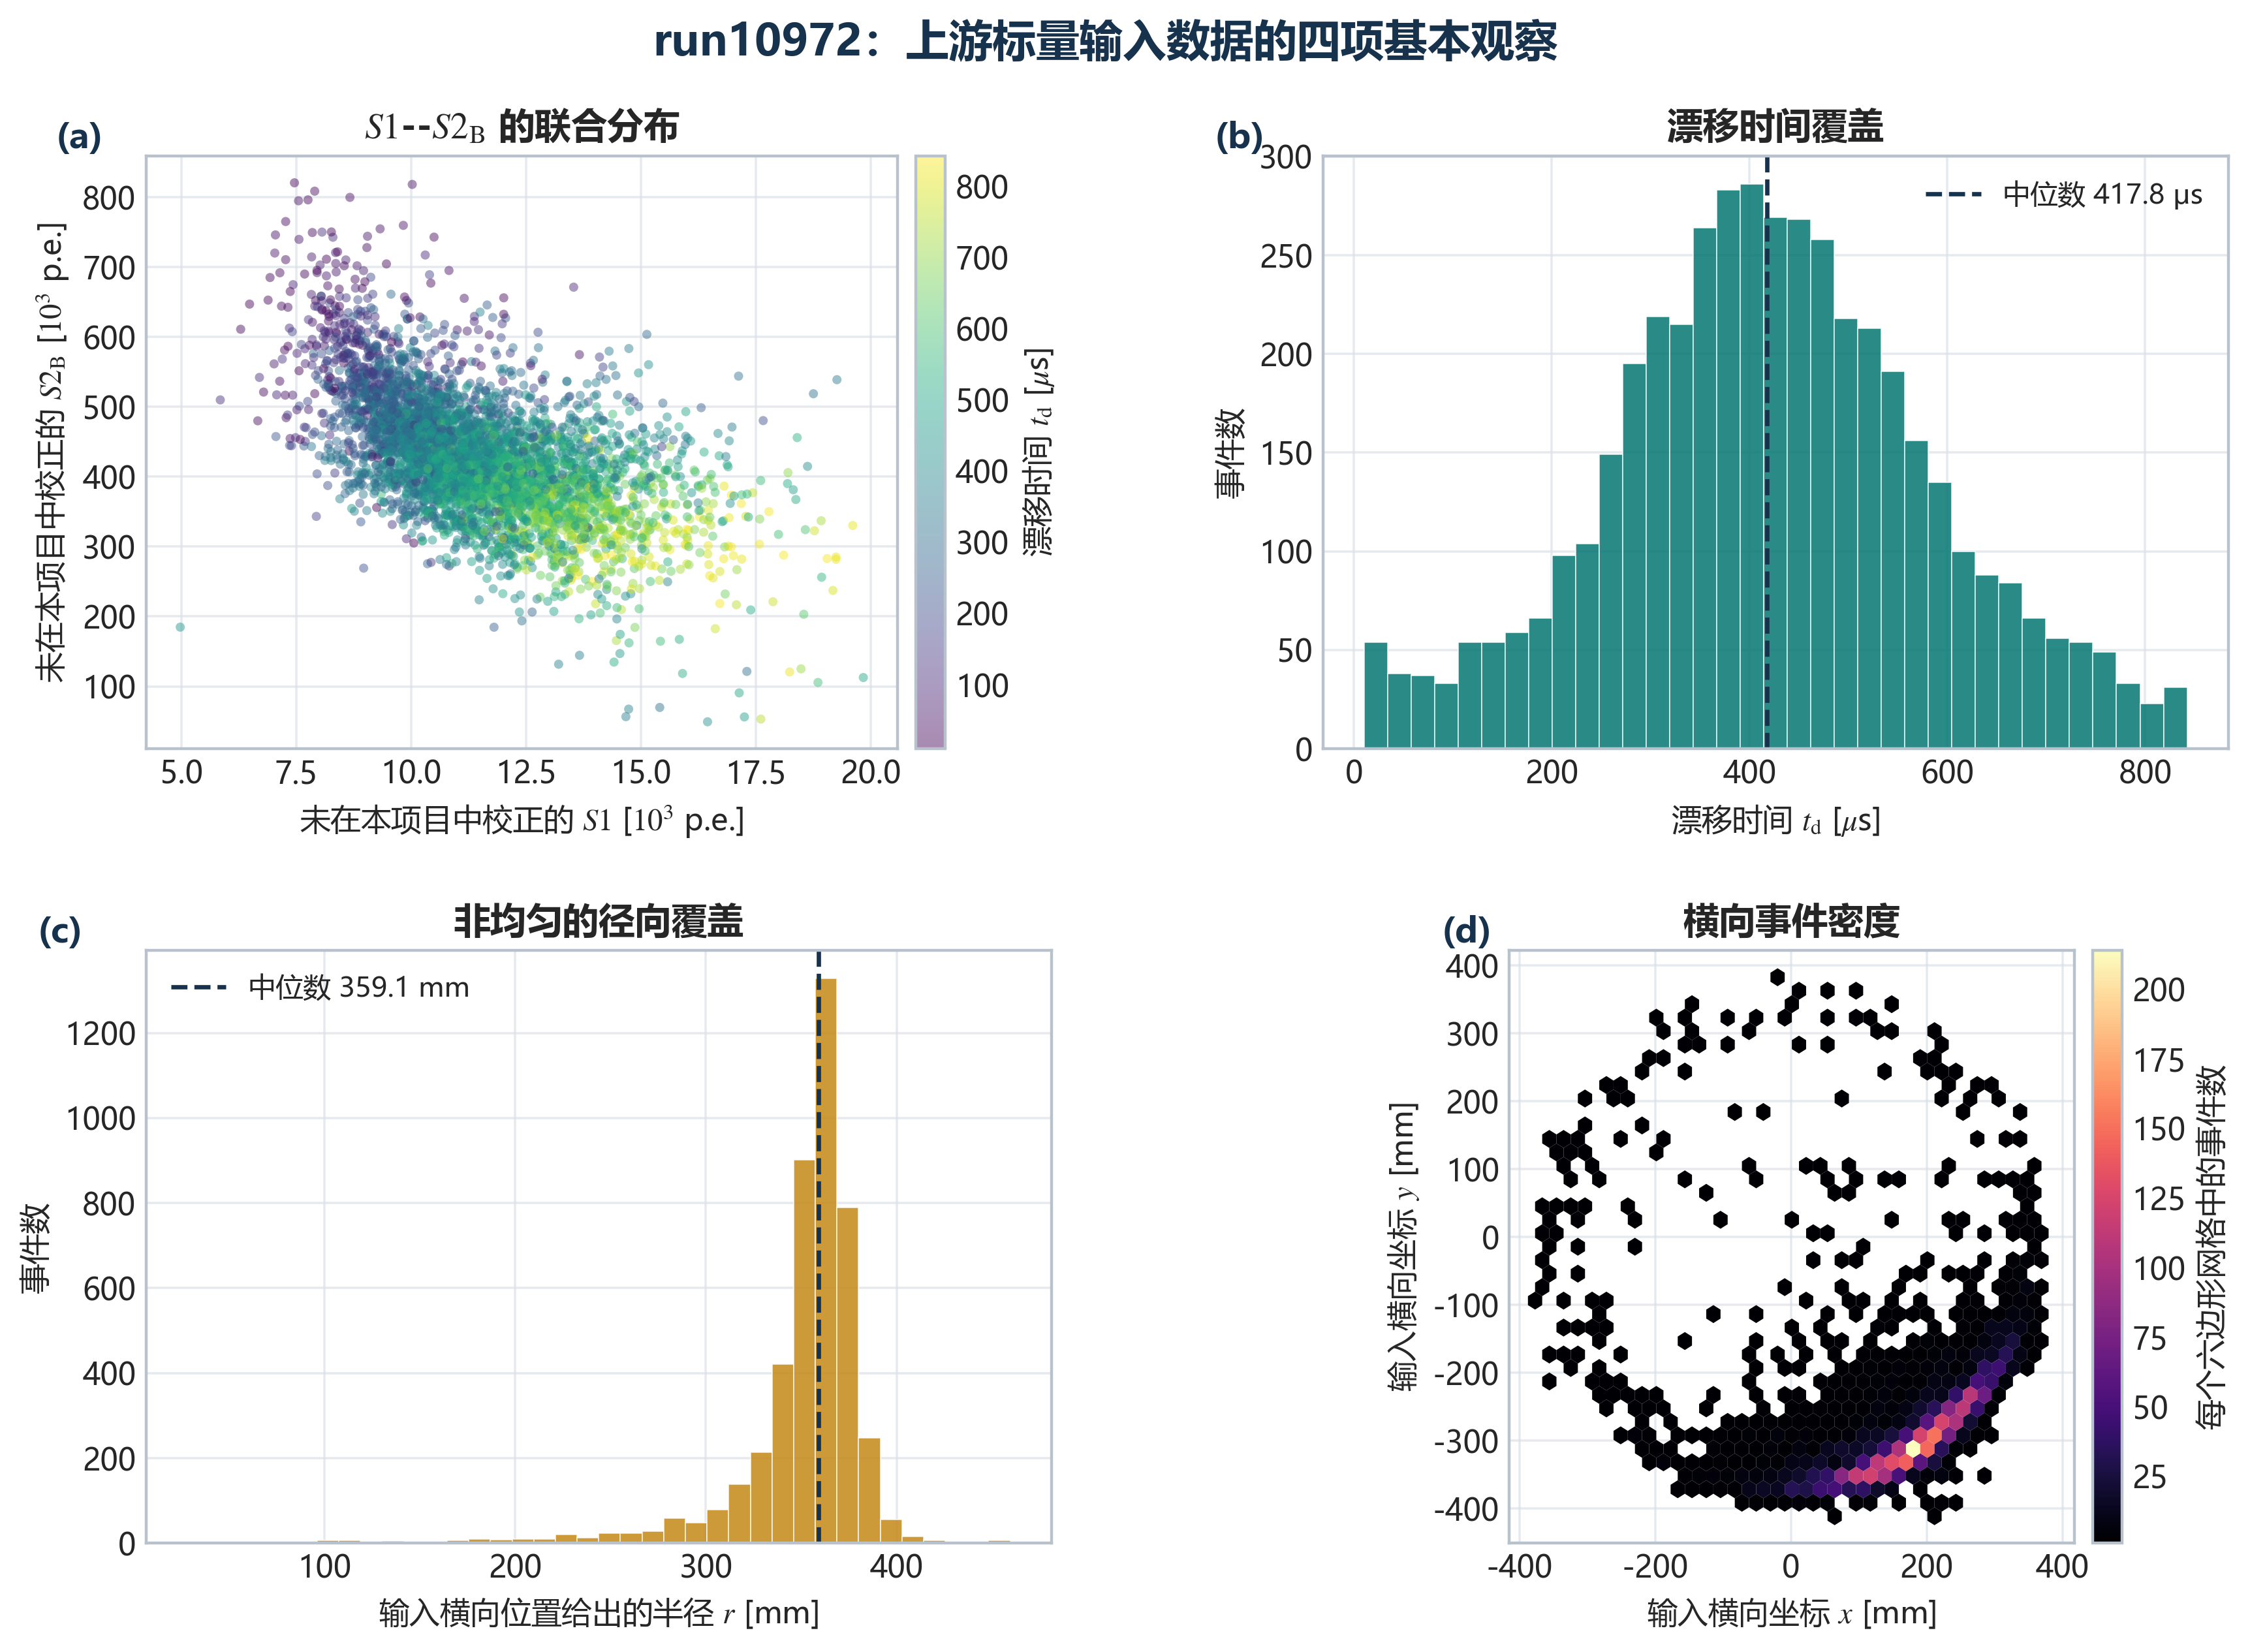
\includegraphics[width=0.96\textwidth]{data_overview.png}
\caption{Run 10972 数据概览：S1--S2B 反相关、漂移时间、横向位置和每文件事件数。}
\end{figure}

左上图表明 S1 与 S2B 存在明显反相关，这是组合能量能够优于单独信号的物理基础。
漂移时间覆盖约 \(0\)--\(\SI{850}{\micro s}\)；横向位置并非均匀填充，
这意味着不能只看整体平均性能，还需要检查位置相关偏差。
每个 \var{fileNumber} 的事件数较少且不相同，因此应把文件身份当作分组元数据，而不是预测特征。

\begin{figure}[H]
\centering
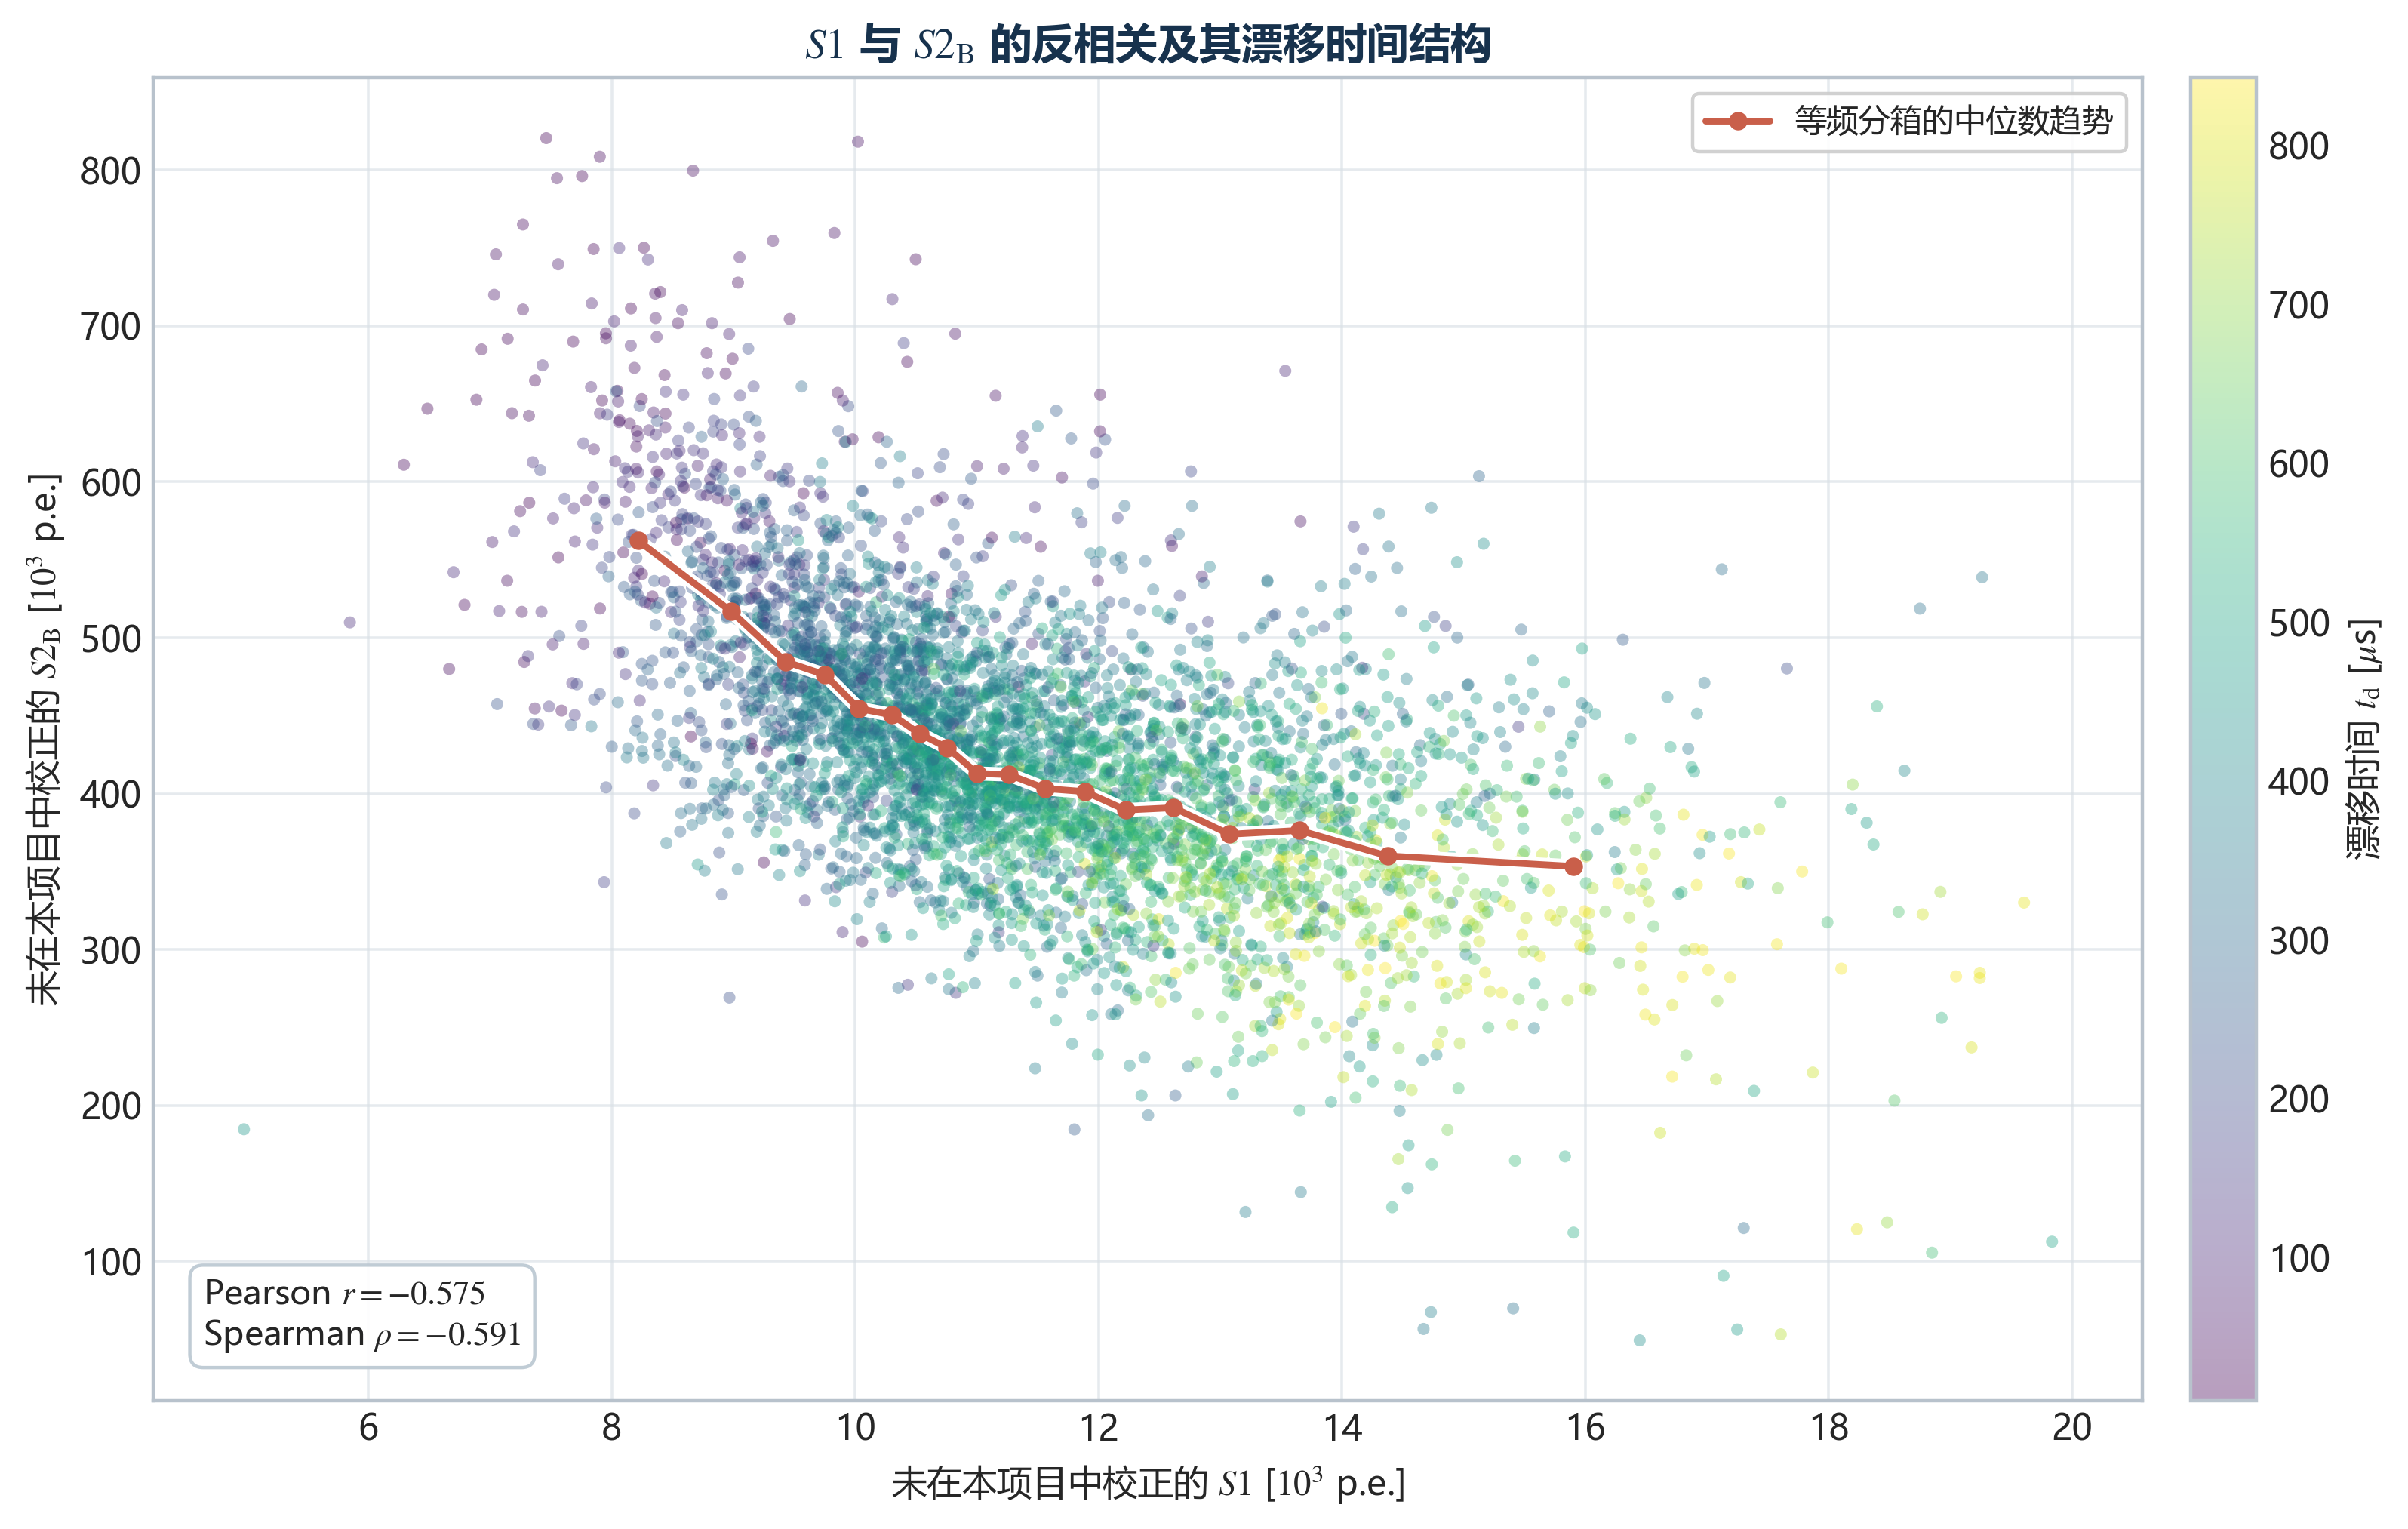
\includegraphics[width=0.92\textwidth]{s1_s2_anticorrelation.png}
\caption{S1--S2B 联合分布及颜色编码的条件变化。主事件带的斜向结构说明两类信号需要联合使用。}
\end{figure}

\subsection{空间覆盖与条件趋势}

\begin{figure}[H]
\centering
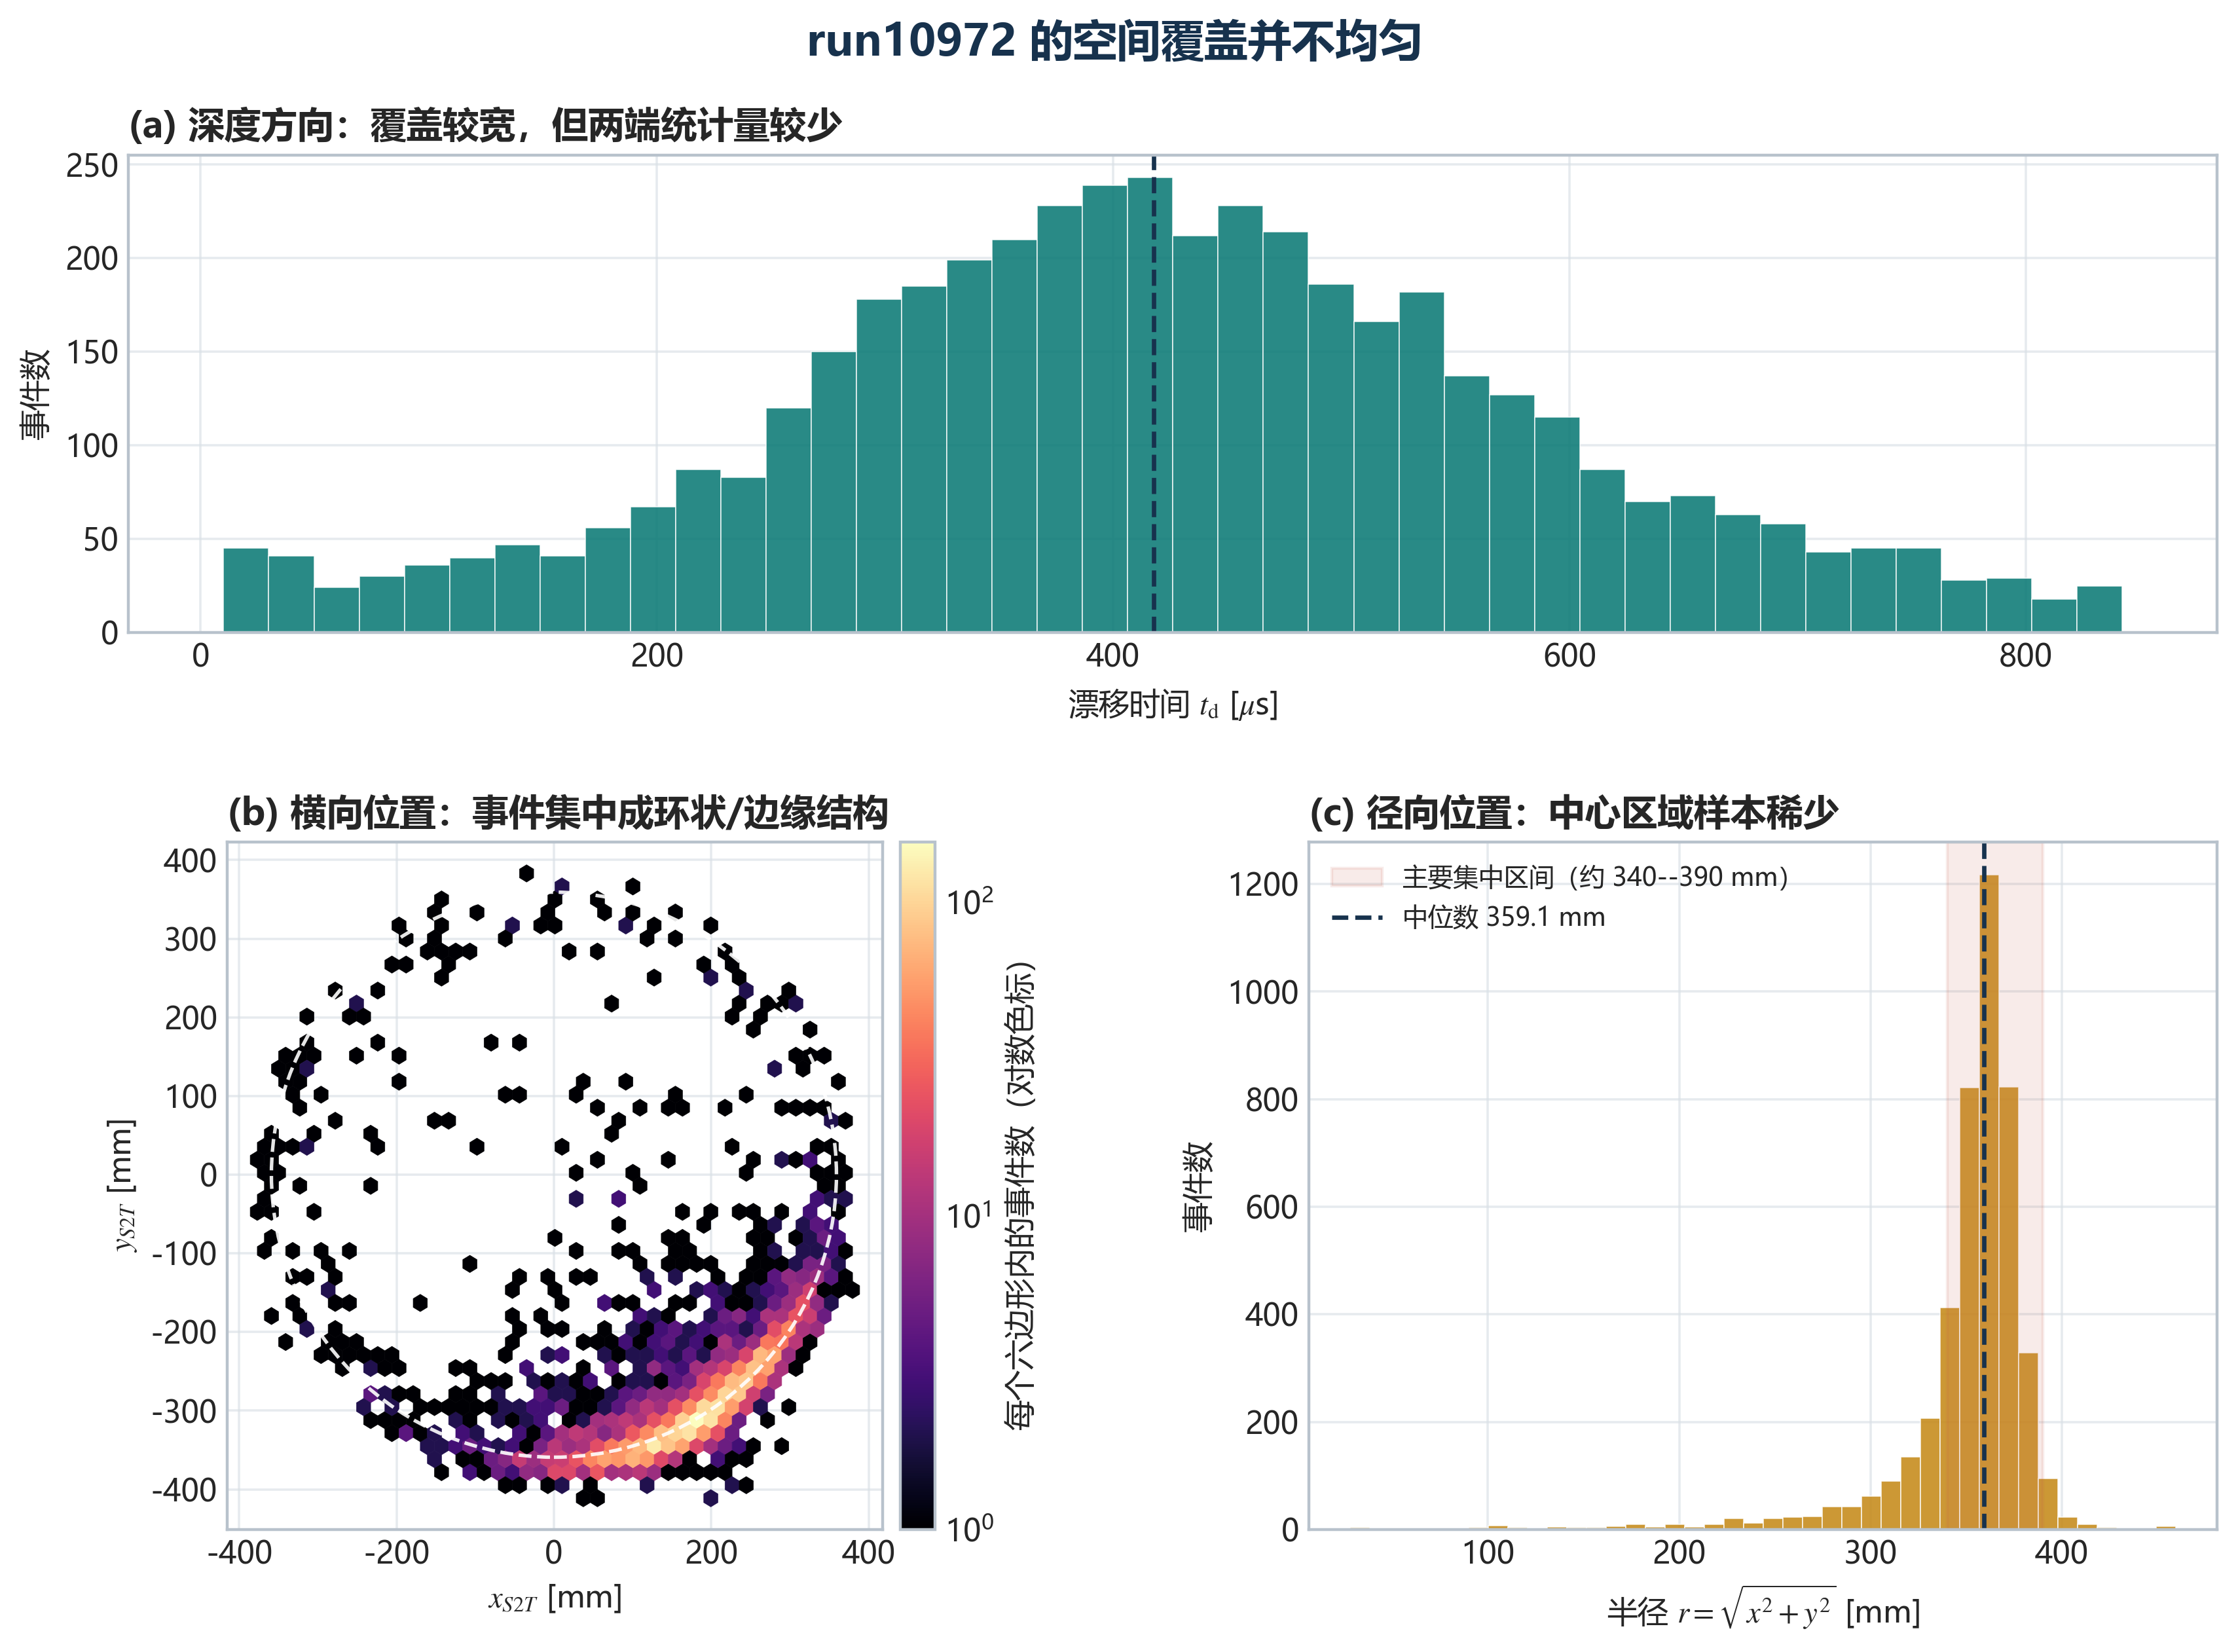
\includegraphics[width=0.93\textwidth]{spatial_coverage.png}
\caption{漂移时间、半径和横向位置覆盖。颜色代表相应条件统计量，而不是模型给出的最终能量。}
\end{figure}

\begin{figure}[H]
\centering
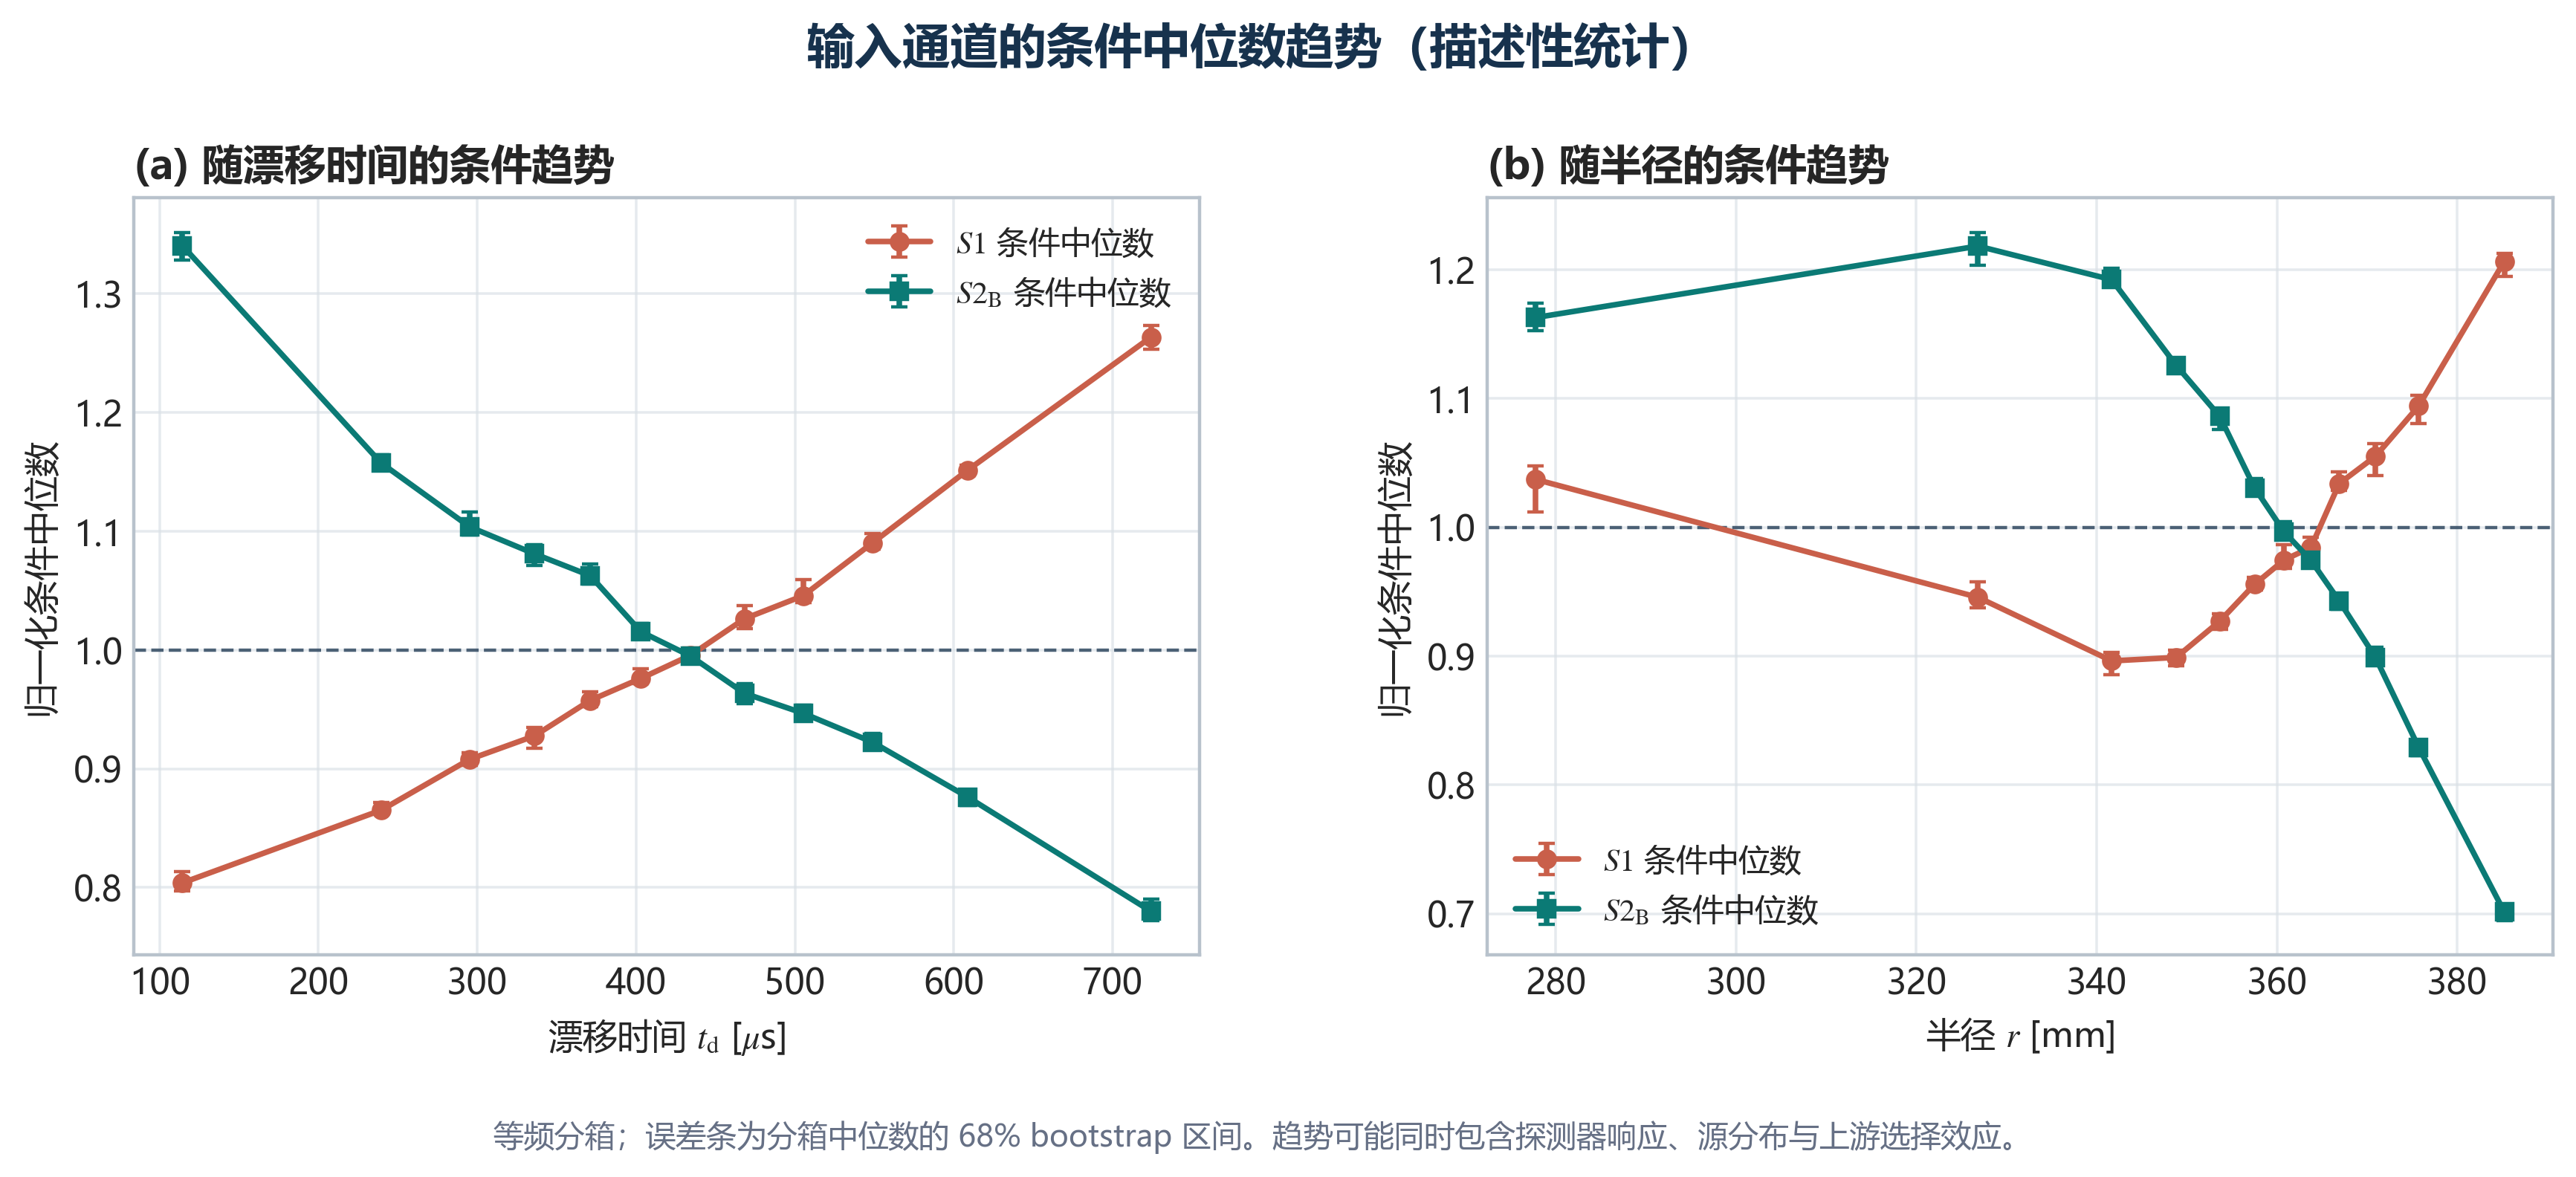
\includegraphics[width=0.96\textwidth]{conditional_trends.png}
\caption{基础信号随漂移时间、半径和横向位置的描述性趋势。}
\end{figure}

这些图只能说明“哪些变量可能值得修正”，不能证明变量具有唯一因果作用，
也不能直接用于选择最终模型。任何修正是否有效，仍需在未见文件块上评价。

\begin{conclusionbox}
数据具有真实的 S1--S2B 反相关、漂移方向和空间非均匀性；
同时采集文件之间可能共享状态。由此决定了两条原则：
修正需要使用受控的物理环境变量，验证需要按完整采集文件隔离。
\end{conclusionbox}

\section{比较对象与统一评价指标}

\subsection{当前线性公式}

当前基础方向为
\begin{equation}
E_0=
\frac{\var{qS1ub_C}}{0.125}
+\frac{\var{qS2Bdesub_C}}{10.58}.
\end{equation}
实际使用的暂定能量写为
\begin{equation}
E_{\mathrm{linear}}=0.0137E_0.
\end{equation}
整体常数不会改变 \(\sigma/\mu\)，但会影响峰中心。验证中任何额外尺度都只能由训练侧确定。

\subsection{已有三次多项式 \texorpdfstring{\(\mathrm{Energy\_cor}\)}{Energy cor}}

\begin{align}
E &=0.0137E_0,\\
E_{\mathrm{cor}}^{\mathrm{legacy}}
&=-1.73706\times10^{-9}E^3
+7.98193\times10^{-6}E^2
+1.07904E-9.22086.
\end{align}

该式是重要基线，但“公式存在”不等于“公式在当前变量和当前数据上最优”。
我们的目标是从数据与变量出发建立可验证的替代修正，并在完全相同的评价口径下比较。

\subsection{固定的 12 种峰拟合协议}

为了避免只挑选最有利的拟合窗口，预先固定四种峰窗口和三种背景形式，共 12 种协议。
主指标为
\begin{equation}
\Rfit=
\operatorname{median}_{p\in\mathcal P}
\left(\frac{\sigma_p}{\mu_p}\right),
\qquad |\mathcal P|=12.
\end{equation}
同时报告非参数核心与尾部宽度：
\begin{align}
\Rsixtyeight&=
\frac{Q_{84.135}-Q_{15.865}}{2Q_{50}},\\
\Rninty&=
\frac{Q_{95}-Q_{5}}{2Q_{50}}.
\end{align}

\begin{notebox}
\(\Rsixtyeight\) 主要描述中间约 68\% 事件的核心宽度；
\(\Rninty\) 覆盖中间 90\% 事件，对长尾和异常事件更敏感。
如果只有拟合核心变窄而 \(\Rninty\) 变差，说明模型可能只是改善了峰中心区域。
\end{notebox}

\section{验证设计：如何防止“看起来很好”的假改善}

\subsection{为什么不能随机拆分事件}

同一 \var{fileNumber} 内的事件可能共享探测器状态、噪声和标定条件。
若随机把同一文件的事件分到训练集和测试集，模型可能识别文件状态，
导致测试结果过于乐观。

Run 10972 被划为五个连续完整文件块：
\[
[0,200),\quad[200,400),\quad[400,600),\quad
[600,800),\quad[800,1000).
\]
每轮锁定一块作为外层测试，其余四块构成训练池。
\var{fileNumber} 只用于分组、追踪和稳定性检查，从不进入预测模型。

\subsection{外层评估与内层选参}

\begin{center}
\begin{tcolorbox}[width=0.92\textwidth,colback=SoftBlue,colframe=DeepBlue,arc=2mm]
\centering
\textbf{锁定外层测试块}
\(\longrightarrow\)
\textbf{训练池内排序变量与选择 \(k\)}
\(\longrightarrow\)
\textbf{用完整训练池重拟合}
\(\longrightarrow\)
\textbf{一次性预测外层测试块}
\end{tcolorbox}
\end{center}

五轮结束后，每个事件恰好获得一次来自未见模型的预测，拼接形成
OOF（out-of-fold）结果。缺失填补、变量尺度、峰中心尺度、变量排名和模型系数
均只能由当前训练侧产生。

\subsection{本项目采用的审计约束}

为了使峰宽改善可以复核，本项目在模型搜索前固定以下约束：
\begin{enumerate}
  \item 完整文件块零重叠；
  \item 外层测试表现不能反向决定基础路径、变量层级或正则强度；
  \item 不使用绝对编号和绝对时间作为预测量；
  \item 固定 12 种拟合协议并报告最坏结果；
  \item 冻结模型后，在新 run 上不重新标定或调参。
\end{enumerate}

\section{探索历程：从基础物理修正到稀疏模型}

\subsection{早期路线解决了什么}

早期报告分别研究了：
\begin{itemize}
  \item S1、S2B、漂移时间和空间坐标的低自由度物理修正；
  \item 通道物理矩阵 A0--A4；
  \item basic response matrix 与组合响应面；
  \item 事件级 OOF、非参数宽度和 bootstrap；
  \item 峰形高斯拟合优度及负结果。
\end{itemize}
这些工作建立了数据读取、变量白名单、OOF 表、响应诊断和报告结构，
但早期事件级随机折不能充分隔离文件状态，因此其性能数值不作为当前 v10 的最终证据。

\begin{figure}[H]
\centering
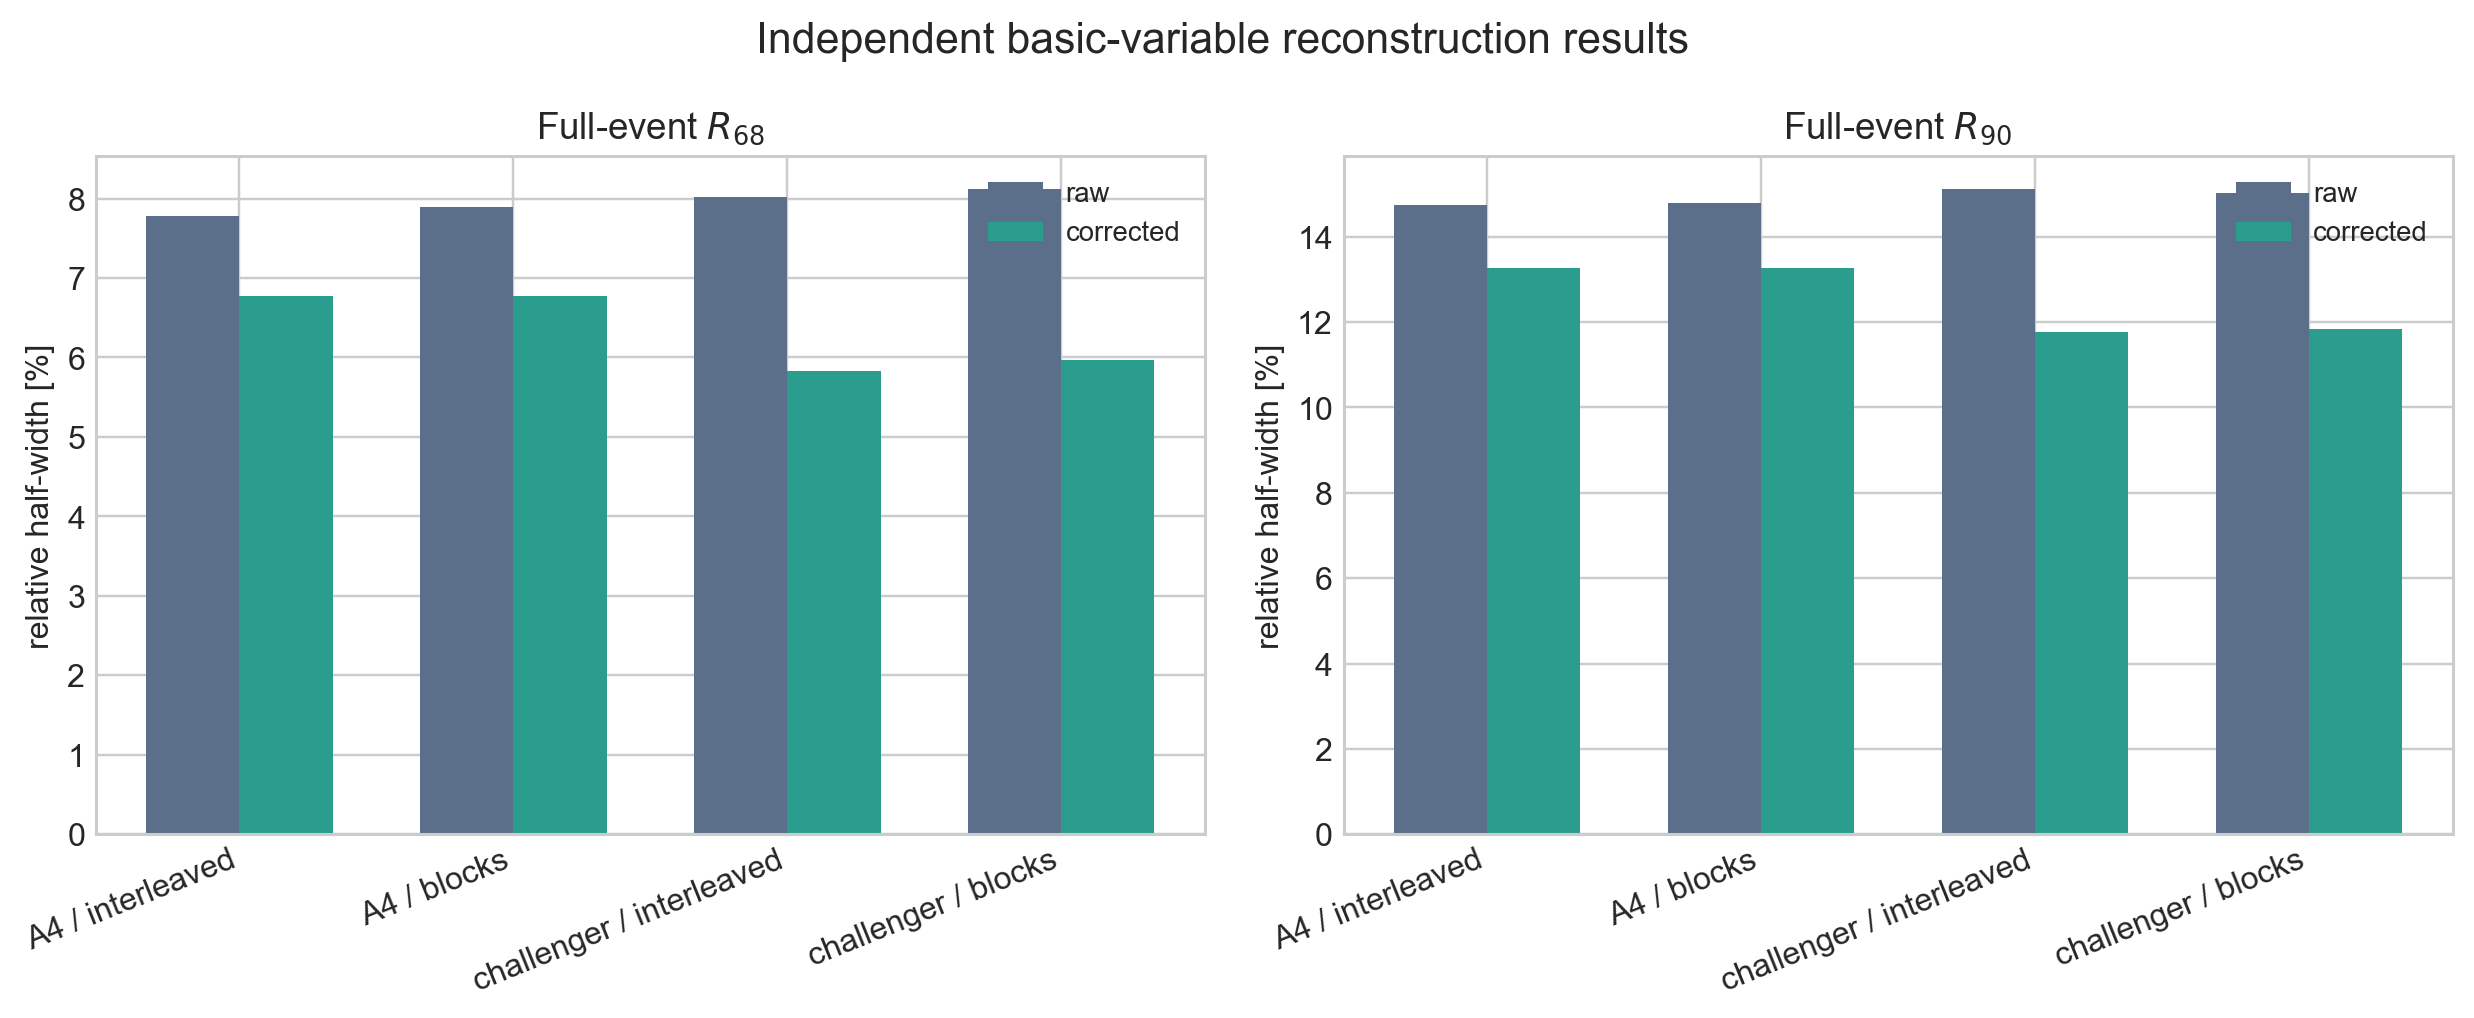
\includegraphics[width=0.86\textwidth]{early_result_summary.png}
\caption{早期基础矩阵与通道物理探索的结果摘要。该图用于说明研究演化，不作为 v10 主结果。}
\end{figure}

\begin{figure}[H]
\centering
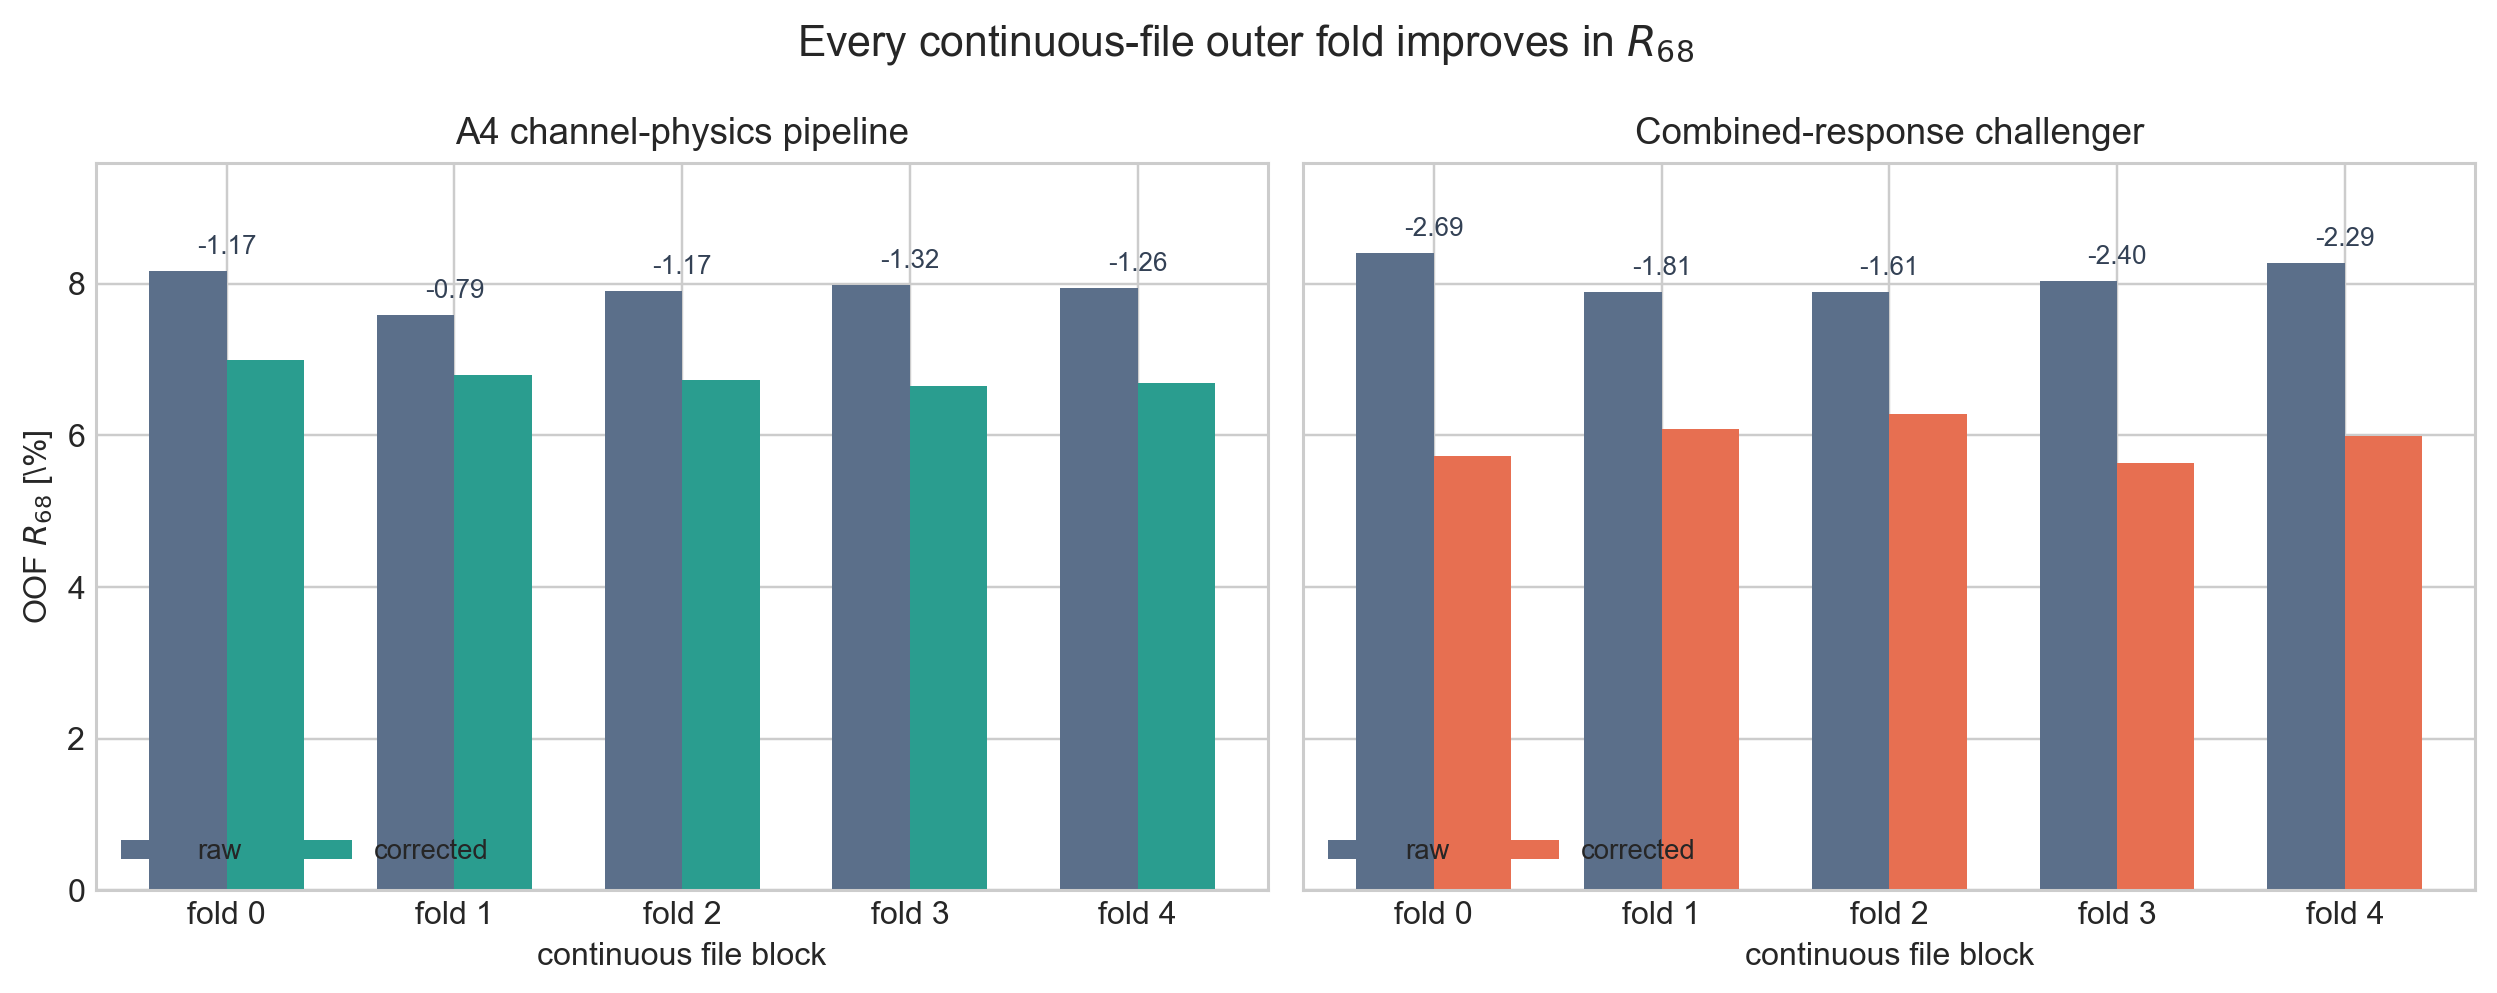
\includegraphics[width=0.88\textwidth]{early_fold_stability.png}
\caption{早期事件折稳定性诊断。它促使后续验证升级为完整 \var{fileNumber} 块隔离。}
\end{figure}

\subsection{v9、v10 与 v11 的核心变化}

v9 已采用平滑样条 Ridge、完整文件块隔离和修正幅度限制，但使用 30 个变量。
老师提出“变量越少越容易控制”，因此 v10 把变量数量本身纳入嵌套选择。
这不是在全数据上看完结果后直接删除变量，而是在每个外层训练池内部独立排序与选择。
v10 的合并 OOF 达到 \(2.7698\%\)，说明环境修正方向有效，但仍未充分利用
上游已经构造的 image charge、更多位置算法和 PMT 图样变量。
v11 因此把基础 S1/S2 路径、变量层级和正则强度一并放入训练侧嵌套选择。

\begin{table}[H]
\centering
\caption{研究路线的角色与证据等级}
\begin{tabularx}{\textwidth}{lC{2.3cm}Y}
\toprule
阶段 & 当前角色 & 主要贡献\\
\midrule
原始数据报告 & 数据依据 & 确认字段、信号相关性、空间覆盖和上游选择边界\\
数据处理报告 & 方法基础 & 建立 split-local、OOF、指标和结果追溯概念\\
早期结果分析 & 探索证据 & 找到有效修正方向，同时暴露峰形和事件折的局限\\
v9 & 模型候选 & 完整文件块分组、低容量平滑修正、30 个变量\\
v10 & 强基线 & 嵌套变量精简、20 个变量、合并 OOF 2.7698\%\\
v11 & 当前主结果 & 训练侧选择 image foundation、64 个受控变量、合并 OOF 0.9973\%\\
\bottomrule
\end{tabularx}
\end{table}

\section{candidate\_v11：模型怎样处理每个事件}

\subsection{模型形式}

v11 不再固定使用单一基础公式，而是在每个外层训练池内部比较五条
S1/S2 基础信号路径。最终冻结路径使用
\var{qS1C_desImageMCPAF_maxS2} 与
\var{qS2BdesC_desImageMCPAF_maxS2}。两路信号先按训练侧中位数归一化：
\begin{equation}
E_{\mathrm{foundation}}
=0.45\frac{S1_{\mathrm{image}}}{\operatorname{median}_{\mathrm{train}}(S1_{\mathrm{image}})}
+0.55\frac{S2_{\mathrm{image}}}{\operatorname{median}_{\mathrm{train}}(S2_{\mathrm{image}})}.
\end{equation}

对选定环境变量构造有限的三次样条基函数
\(\phi(\mathbf{x})\)，使用 Ridge 回归预测基础能量的对数偏差：
\begin{equation}
\widehat{\delta}_{\mathrm{raw}}(\mathbf{x})
=\beta^{\mathsf T}\phi(\mathbf{x}).
\end{equation}
Ridge 目标可写为
\begin{equation}
\widehat{\beta}
=\arg\min_{\beta}
\left[
\sum_{i\in\mathrm{train}}
\left(y_i-\beta^{\mathsf T}\phi(\mathbf{x}_i)\right)^2
+\alpha\lVert\beta\rVert_2^2
\right],
\qquad \alpha=0.01.
\end{equation}

为了避免硬截断产生边界堆积，使用平滑修正上限
\begin{equation}
\widehat{\delta}
=c\tanh\left(\frac{\widehat{\delta}_{\mathrm{raw}}}{c}\right),
\qquad c=0.10.
\end{equation}
最终重建能量为
\begin{equation}
E_{\mathrm{v11}}
=K E_{\mathrm{foundation}}\exp(-\widehat{\delta}),
\end{equation}
其中 \(K\) 只由当前训练侧确定。

\subsection{这不是决策树}

v11 不是决策树、随机森林或神经网络。它可以理解为：
\begin{enumerate}
  \item 先在训练侧选择更合适的 S1/S2 image foundation；
  \item 再观察位置、漂移和脉冲图样等变量；
  \item 用平滑曲线估计该探测器状态通常会让基础能量偏高还是偏低；
  \item 对基础能量做一个受限的小幅乘法修正。
\end{enumerate}
选择这种模型是为了在 4499 个有效事件上控制容量、保持可审计性，并减少极端外推。

\subsection{基础路径、变量层级与正则如何确定}

\begin{figure}[H]
\centering
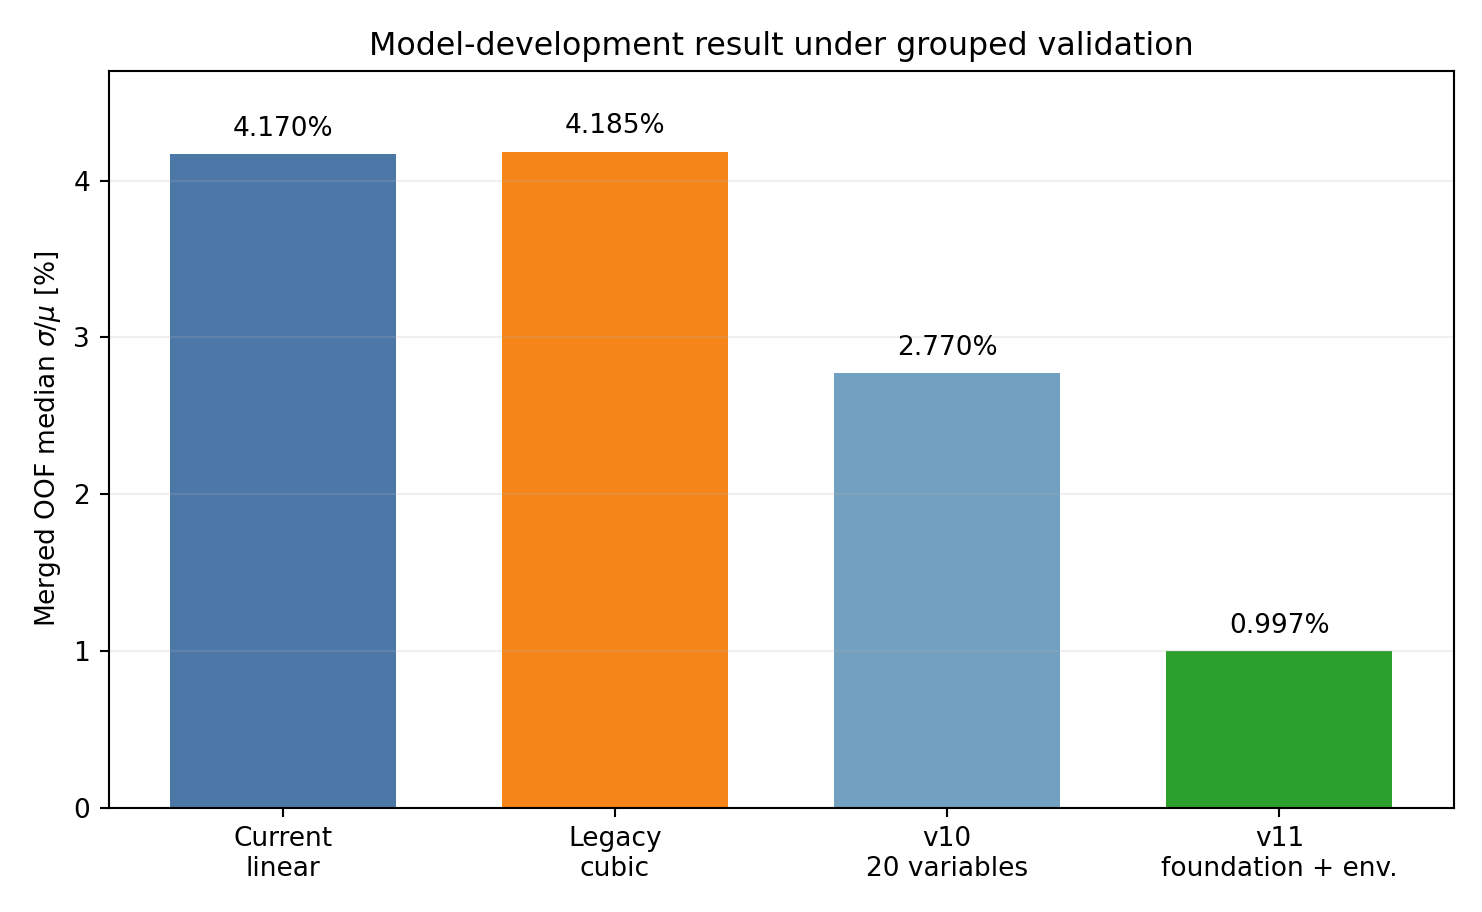
\includegraphics[width=0.82\textwidth]{v11_model_progress.png}
\caption{在完整文件块验证口径下，当前线性公式、已有三次式、v10 与 v11 的合并 OOF 结果。}
\end{figure}

每个外层训练池内部先比较五条基础 S1/S2 路径，再比较三层变量集合：
32 个 core 变量、48 个 detector 变量和 64 个 environment 变量；
最后比较
\[
\alpha\in\{10^{-4},10^{-2},1,30,100\}.
\]
五个外层流程分别选择 image-derived 基础路径，并在 detector 与 environment
层之间选择；最终冻结身份由外层流程的多数选择确定为
image foundation、64 个变量与 \(\alpha=0.01\)。
外层测试块从未参与这些选择。

\section{关键变量与响应信息}

\begin{landscape}
\begin{figure}[H]
\centering
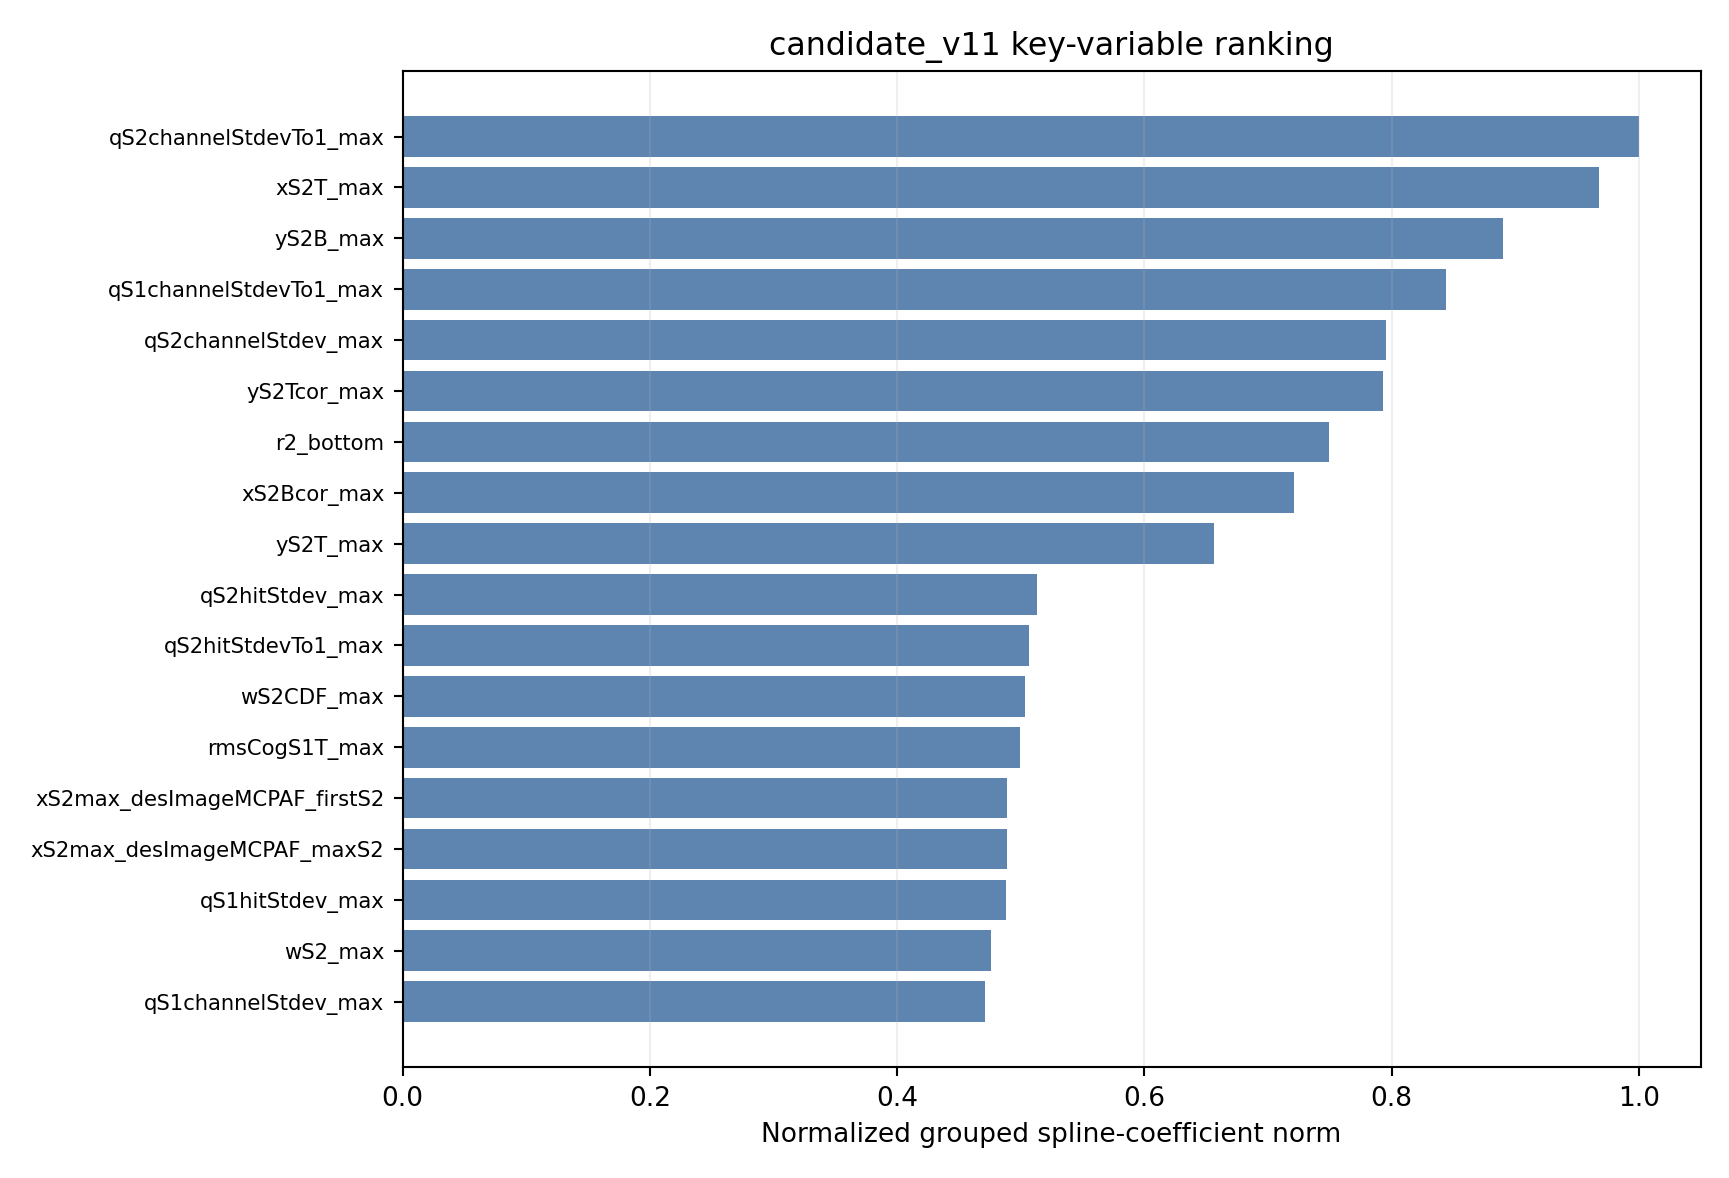
\includegraphics[width=0.88\linewidth]{v11_feature_importance.png}
\caption{v11 冻结模型的分组样条系数范数排序。
该排序用于诊断模型依赖，不表示唯一因果贡献。}
\end{figure}
\end{landscape}

\begin{table}[H]
\centering
\caption{排名前五的关键变量}
\begin{tabularx}{\textwidth}{C{1cm}lY C{2cm}}
\toprule
排名 & 变量 & 可作出的物理解读 & 相对重要性\\
\midrule
1 & \var{qS2channelStdevTo1_max} & S2 通道图样的相对离散程度 & 1.000\\
2 & \var{xS2T_max} & S2 顶阵列重建的横向位置 & 0.968\\
3 & \var{yS2B_max} & S2 底阵列重建的横向位置 & 0.890\\
4 & \var{qS1channelStdevTo1_max} & S1 通道图样的相对离散程度 & 0.844\\
5 & \var{qS2channelStdev_max} & S2 通道电荷的绝对离散程度 & 0.796\\
\bottomrule
\end{tabularx}
\end{table}

排名显示，v11 的主要增益来自两类信息：PMT 通道图样与多套横向位置重建。
其中绝对通道离散度可能携带总电荷尺度信息，是 v11 比 v10 更强、同时也更需要
独立 run 审计的原因之一。模型不会修改输入变量本身，而是根据这些变量所代表的
探测器响应状态对 foundation energy 作受限修正。

\section{核心结果：四套 corrected energy 的统一比较}

\subsection{一维能谱}

\begin{figure}[H]
\centering
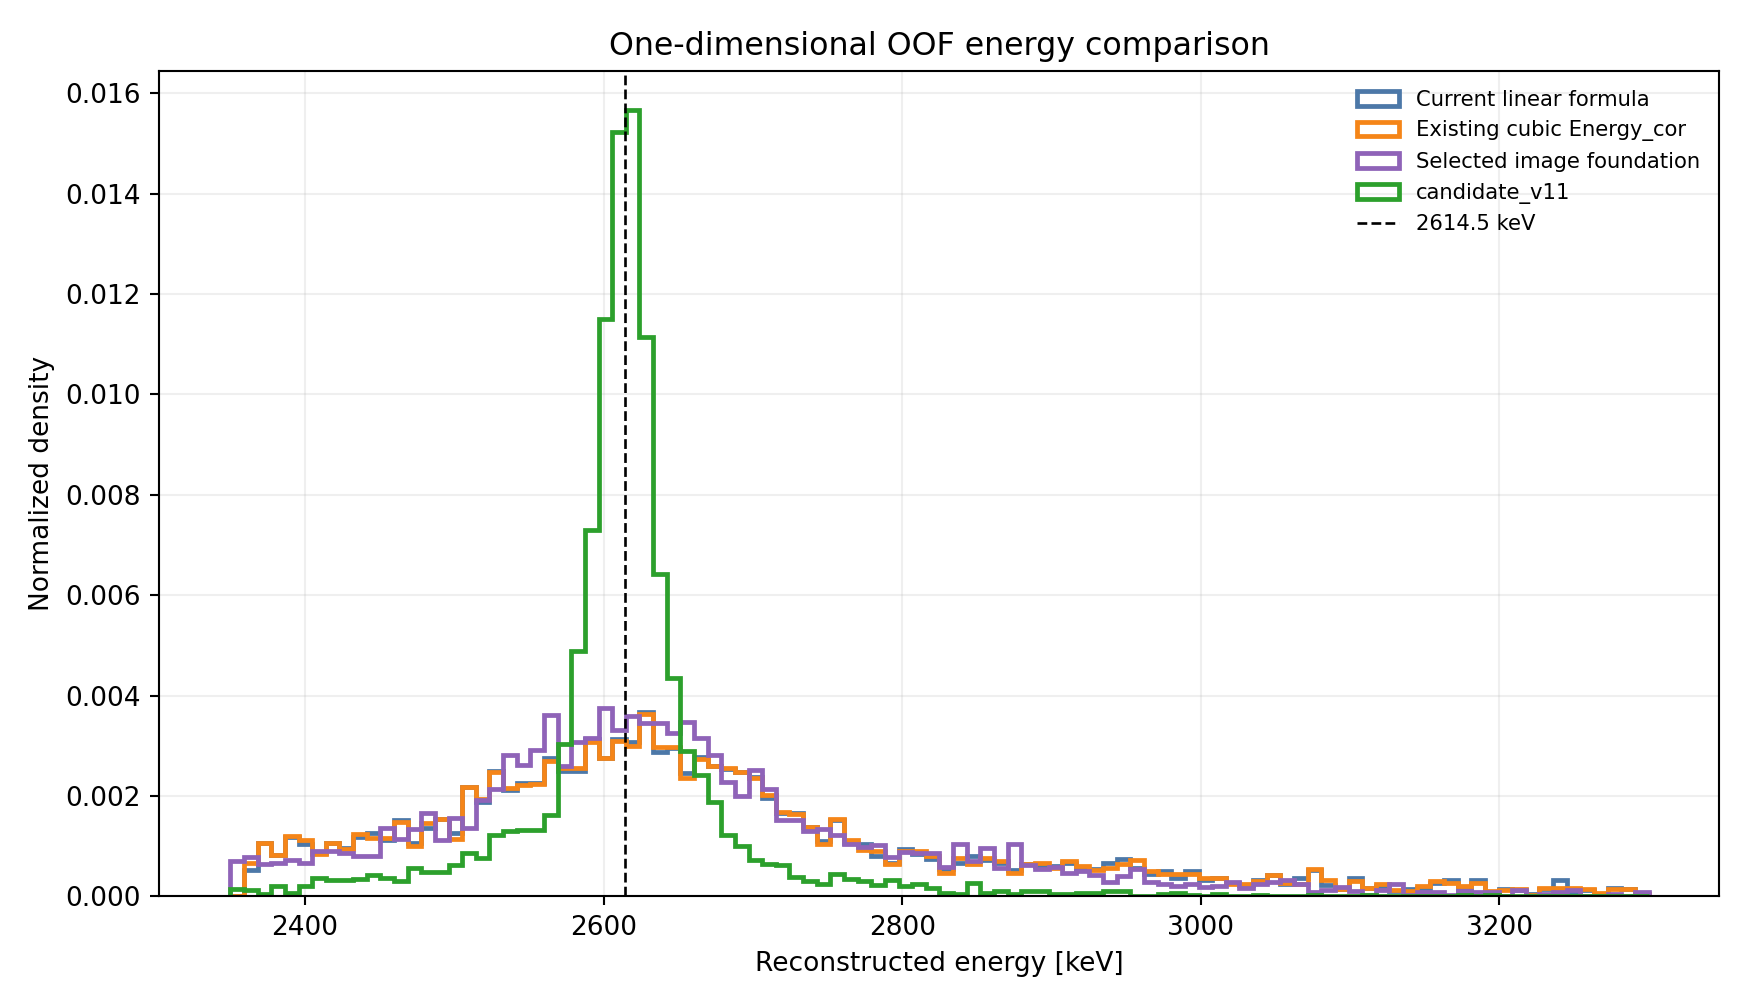
\includegraphics[width=0.93\textwidth]{v11_energy_1d.png}
\caption{四种重建方法在同一批合并 OOF 事件上的归一化一维能谱。
v11 的中心峰显著更窄，但仍保留非高斯尾部。}
\end{figure}

\begin{table}[H]
\centering
\caption{合并 OOF 的统一指标}
\begin{tabular}{lrrrr}
\toprule
方法 & \(\Rfit\) 中位数 & 最差协议 & \(\Rsixtyeight\) & \(\Rninty\)\\
\midrule
当前线性公式 & 4.1696\% & 4.3869\% & 6.7861\% & 13.0694\%\\
已有三次式 \var{Energy_cor} & 4.1847\% & 4.4404\% & 6.8242\% & 13.1471\%\\
训练侧选择的 foundation & 3.8552\% & 6.4701\% & 6.2078\% & 12.5692\%\\
\textbf{candidate\_v11} & \textbf{0.9973\%} & \textbf{1.0427\%}
& \textbf{1.3674\%} & \textbf{4.2483\%}\\
\bottomrule
\end{tabular}
\end{table}

相对当前线性公式，
\begin{equation}
1-\frac{0.9973}{4.1696}=76.1\%.
\end{equation}
相对已有三次式，
\begin{equation}
1-\frac{0.9973}{4.1847}=76.2\%.
\end{equation}
核心宽度与尾部宽度同时下降，说明改善不只发生在高斯峰中心。

\subsection{五个未见文件块}

\begin{figure}[H]
\centering
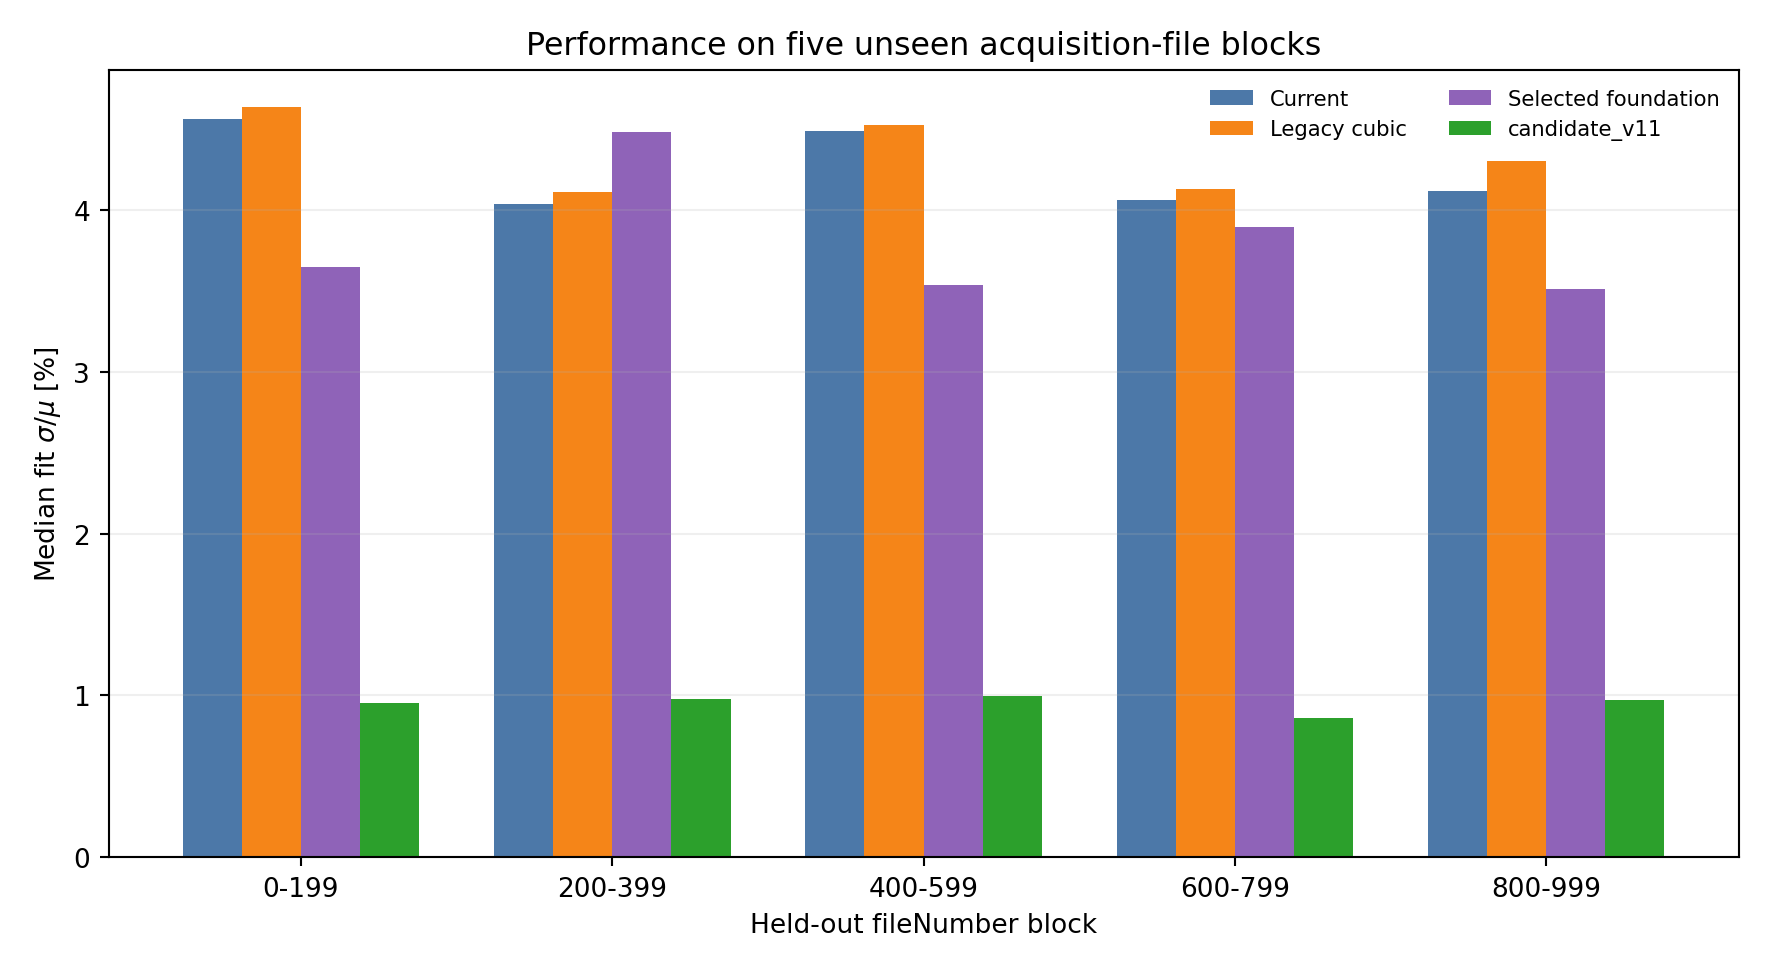
\includegraphics[width=0.9\textwidth]{v11_outer_blocks.png}
\caption{五个完整外层文件块上的 \(\Rfit\)。每个绿色柱均来自未见该文件块的模型。}
\end{figure}

\begin{table}[H]
\centering
\caption{逐外层文件块结果}
\begin{tabular}{lrrrr}
\toprule
\var{fileNumber} & 当前线性 & 已有三次式 & foundation & v11\\
\midrule
0--199 & 4.5616\% & 4.6349\% & 3.6460\% & \textbf{0.9523\%}\\
200--399 & 4.0356\% & 4.1127\% & 4.4838\% & \textbf{0.9774\%}\\
400--599 & 4.4918\% & 4.5284\% & 3.5345\% & \textbf{0.9990\%}\\
600--799 & 4.0605\% & 4.1323\% & 3.8948\% & \textbf{0.8595\%}\\
800--999 & 4.1179\% & 4.3011\% & 3.5104\% & \textbf{0.9701\%}\\
\midrule
五块中位数 & 4.1179\% & 4.3011\% & 3.6460\% & \textbf{0.9701\%}\\
\bottomrule
\end{tabular}
\end{table}

五个文件块全部改善，比只报告合并能谱更有说服力：
它说明结果没有由单一采集时段支撑。

\subsection{v9、v10 与 v11}

\begin{table}[H]
\centering
\caption{模型版本演化}
\begin{tabularx}{0.92\textwidth}{lC{2cm}C{3cm}C{3cm}Y}
\toprule
版本 & 变量数 & 合并 OOF \(\Rfit\) & 五块中位数 & 解释\\
\midrule
v9 & 30 & 2.7690\% & 2.6287\% & 完整平滑模型\\
v10 & 20 & 2.7698\% & 2.5731\% & 稀疏环境修正强基线\\
v11 & 64 & 0.9973\% & 0.9701\% & 搜索基础路径并加入完整图样和环境信息\\
\bottomrule
\end{tabularx}
\end{table}

\clearpage
\begin{landscape}
\section{二维空间、修正幅度与数值安全}
\begin{figure}[H]
\centering
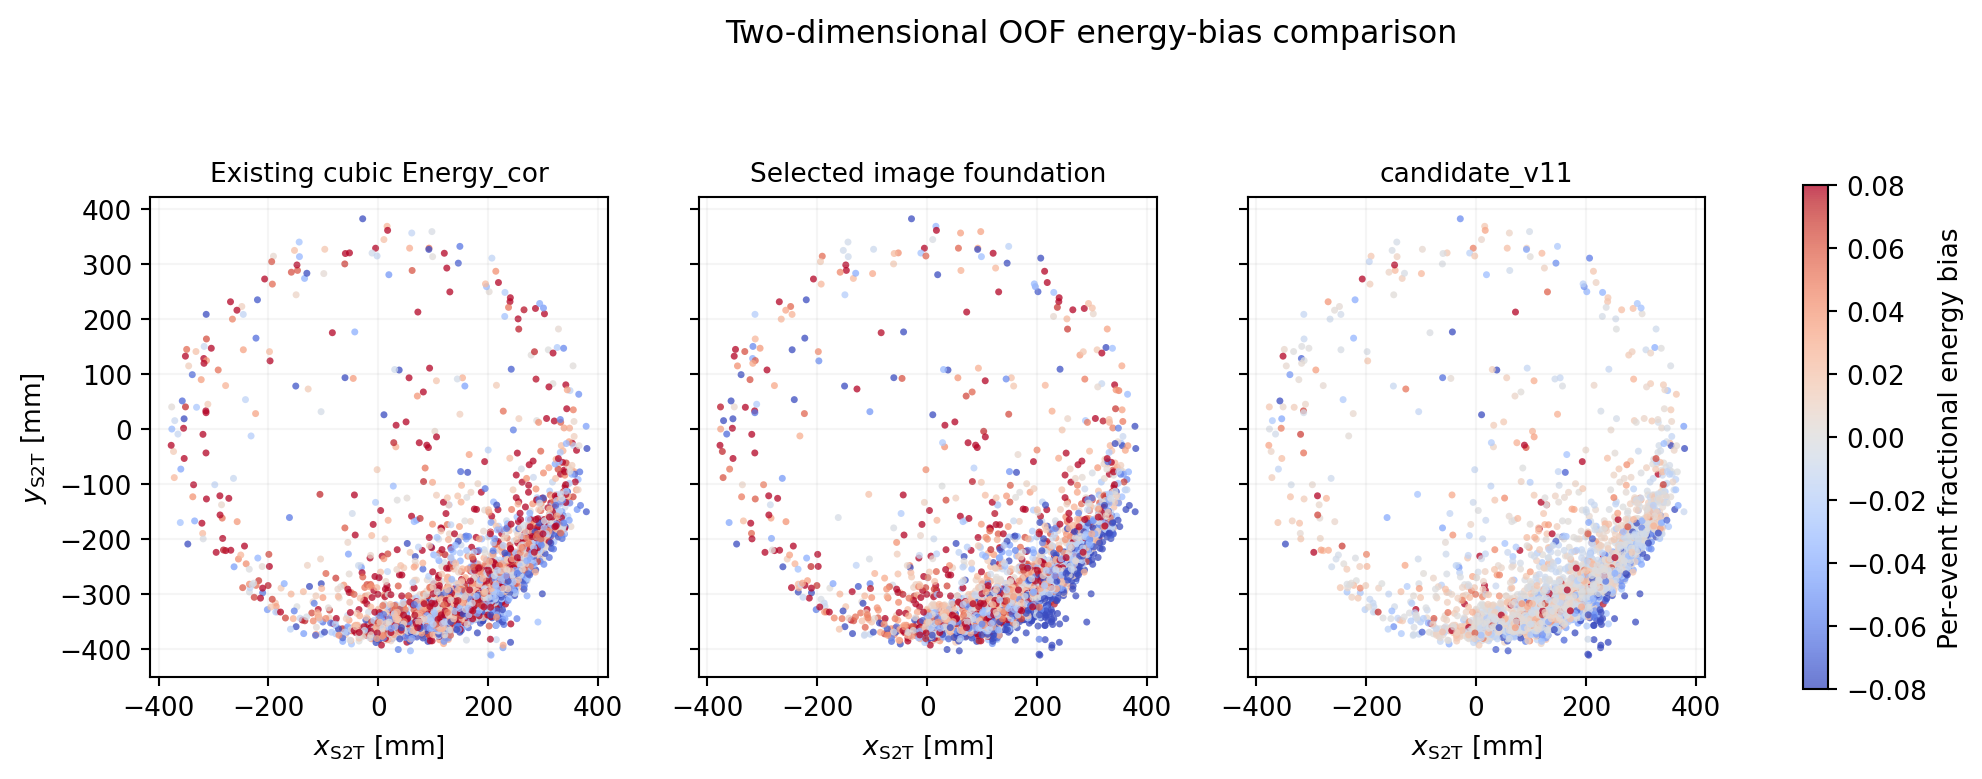
\includegraphics[width=0.9\linewidth]{v11_xy_bias.png}
\caption{已有三次式、训练侧选择的 foundation 与 v11 的 \(x-y\) 逐事件偏差图。
颜色表示相对 \(\SI{2614.5}{keV}\) 的逐事件偏差，不是事件密度。}
\end{figure}
\end{landscape}

二维图的目标不是寻找“最漂亮的颜色”，而是回答三个问题：
\begin{enumerate}
  \item 是否存在某个空间区域系统性偏高或偏低；
  \item v11 是否减弱已有三次式与 foundation 的空间结构；
  \item 改善是否只来自事件密集的局部区域。
\end{enumerate}
当前图显示 v11 的整体偏差范围更集中，但边缘与稀疏区域仍应在新 run 中单独检查。

\begin{figure}[H]
\centering
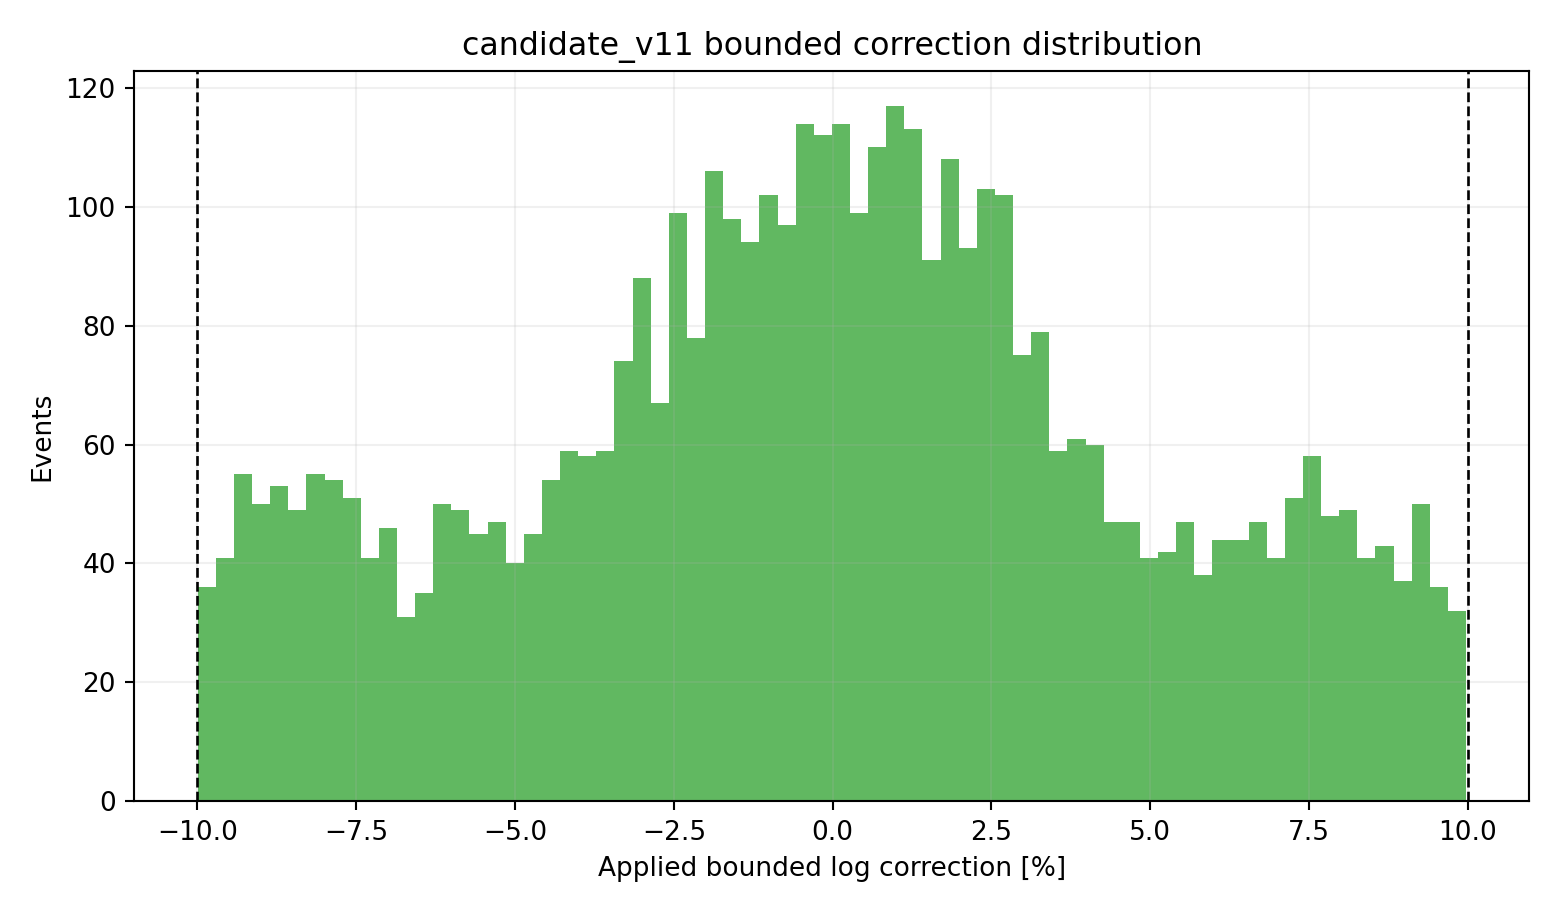
\includegraphics[width=0.87\textwidth]{v11_correction.png}
\caption{v11 的单事件对数修正分布。虚线为平滑上限 \(\pm0.10\)。}
\end{figure}

全部 4499 个有效事件的预测均为有限正值；
接近修正上限的事件比例约 \(2.60\%\)。
这说明模型没有依靠让大批事件触顶来压窄峰，但尾部事件仍需要重点复核。

\begin{table}[H]
\centering
\caption{当前验收状态}
\begin{tabularx}{0.92\textwidth}{Y C{2.4cm}Y}
\toprule
检查 & 状态 & 说明\\
\midrule
五个外层块均优于当前公式 & \pass & 逐块结果全部改善\\
五个外层块均优于已有三次式 & \pass & 逐块结果全部改善\\
12 种协议均成功 & \pass & 合并 OOF 四路线均为 12/12\\
有限且为正 & \pass & 4499 个有效事件全部通过\\
修正幅度受限 & \pass & 平滑上限 0.10，近上限比例约 2.60\%\\
独立新 run & \pending & 尚未取得老师的新数据\\
峰形拟合优度 & \pending & v11 中位 \(p\) 值数值上趋近零，单高斯模型明显不充分\\
\bottomrule
\end{tabularx}
\end{table}

\section{为什么 v11 能从 2.77\% 降到约 1.00\%}

这次下降不是由单一参数造成，而是三项改变共同作用：
\begin{enumerate}
  \item \textbf{基础信号路径改变：}
  训练侧不再固定使用 \var{qS1ub_C} 与 \var{qS2Bdesub_C}，
  而是在多条基础路径中选择 image-derived S1/S2 组合；
  \item \textbf{响应信息更完整：}
  从 v10 的 20 个变量扩展到 64 个受控变量，
  加入多套横向位置、脉冲形状、PMT 通道图样与事件环境；
  \item \textbf{模型容量增加但仍受限：}
  训练侧选择 \(\alpha=0.01\)，比 v10 的 \(\alpha=100\) 更灵活，
  但单事件对数修正仍由 \(\pm0.10\) 平滑限制。
\end{enumerate}

\subsection{为什么不能只看 0.9973\%}

更强模型也带来更高审计要求：
\begin{itemize}
  \item 绝对通道离散度等变量可能携带总电荷尺度，跨能量或跨 run 外推风险更高；
  \item 合并 OOF 的 \(\Rninty=4.2483\%\) 仍明显大于核心宽度，尾部没有消失；
  \item 峰形拟合 \(p\) 值趋近零，说明“极窄单高斯”不能完整描述能谱；
  \item 当前五块仍来自同一个 Run 10972，不能替代独立运行期；
  \item 若新 run 上性能明显退化，应保留失败结果，而不是利用新 run 继续调参。
\end{itemize}

\begin{scopebox}
0.9973\% 是严格文件块隔离下的内部 OOF 结果，是真实的阶段性进展；
但在独立新 run 通过以前，它仍只能称为 candidate\_v11，而不能称为最终能量分辨率。
\end{scopebox}

\section{老师在新数据上怎样运行}

\subsection{冻结交付包}

当前交付包为
\var{PandaX_candidate_v11_blindtest_FINAL_20260731.zip}，包含：
\begin{itemize}
  \item 冻结模型 \var{candidate_v11.joblib}；
  \item 应用脚本 \var{apply_foundation_environment_v11.py}；
  \item Linux 与 Windows 一键运行脚本；
  \item 依赖环境、模型卡和 SHA-256；
  \item 输入字段检查与四路线统一评价。
\end{itemize}

模型文件 SHA-256 为
\begin{center}
\small\ttfamily
eb75c52cdea1d039fa792bb1073451feda61cc4acbd07a8db2150aec1fc1e5bd
\end{center}

\subsection{运行方式}

Linux:
\begin{verbatim}
conda env create -f environment.yml
conda activate pandax-eres-validation
chmod +x run_validation.sh
./run_validation.sh /path/to/new_run_scalar.txt
\end{verbatim}

Windows:
\begin{verbatim}
run_validation.bat C:\path\to\new_run_scalar.txt
\end{verbatim}

程序输出：
\begin{itemize}
  \item \var{validation_summary.json}：四路线汇总指标；
  \item \var{validation_protocols.csv}：12 种协议逐项结果；
  \item \var{validation_events.csv}：逐事件能量、修正量和身份列。
\end{itemize}

\subsection{独立盲测纪律}

首次运行后应原样保存输出。在报告第一次结果之前，不允许：
\begin{itemize}
  \item 用新 run 重新训练或选择变量；
  \item 根据新峰中心重新标定；
  \item 改变峰窗口、背景形式或删除表现不好的事件；
  \item 因结果不理想而立即调参后仍称其为盲测。
\end{itemize}

\section{当前不足、风险与下一步}

\subsection{当前仍不能声称什么}

\begin{enumerate}
  \item 不能声称 v11 已经是数学意义或物理意义上的全局最优模型；
  \item 不能声称 Run 10972 内的改善会完整迁移到其他 run；
  \item 不能声称变量重要性就是微观因果贡献；
  \item 不能把合并 OOF 的 0.9973\% 称为独立数据结果；
  \item 不能忽略峰形拟合优度仍很小这一问题。
\end{enumerate}

\subsection{为什么拟合优度仍然很差}

虽然 \(\sigma/\mu\) 明显下降，v11 的拟合 \(p\) 值在数值上趋近零。
可能原因包括：
\begin{itemize}
  \item 峰并非单一高斯，存在非高斯尾部；
  \item 上游选择中仍混有背景或不同事件成分；
  \item 不同采集状态混合产生轻微多峰或偏斜；
  \item 统计模型的背景形式仍过于简单。
\end{itemize}
因此后续应尝试 Crystal Ball、双侧尾部或信号加背景的更合理峰形模型，
但拟合协议必须在查看独立新 run 前冻结。

\subsection{建议执行顺序}

\begin{enumerate}
  \item \textbf{先做独立新 run 盲测：}这是当前最有信息量的一步；
  \item \textbf{补齐分簇 bootstrap：}以 \var{fileNumber} 为簇比较四路线差值；
  \item \textbf{补齐分层消融：}定量比较位置、形状、PMT 图样和环境四类信息；
  \item \textbf{加入负对照：}验证绝对 ID/时间不会形成捷径；
  \item \textbf{改进峰形模型：}在不改变 OOF 预测的前提下复核非高斯尾部；
  \item \textbf{若盲测失败：}报告失败并建立 v12，新旧证据目录分离。
\end{enumerate}

\section{最终结论}

\begin{conclusionbox}
\begin{enumerate}
  \item 我们已从 Run 10972 的上游标量数据出发，建立独立于已有公式参数的能量修正流程；
  \item v11 在训练侧选择 image foundation、64 个变量与 \(\alpha=0.01\)；
  \item 合并 OOF \(\Rfit\) 为 0.9973\%，相对当前线性公式改善约 76.1\%；
  \item 五个完整未见文件块全部改善，核心宽度 \(\Rsixtyeight\) 与尾部宽度
  \(\Rninty\) 同时下降；
  \item 关键变量主要来自 S1/S2 通道图样和多套横向位置重建；
  \item 已完成一维能谱、二维 \(x-y\)、关键变量、修正幅度和数值安全检查；
  \item 已生成可供老师直接运行的冻结盲测包；
  \item 下一项决定性工作是使用完全独立的新 run，一次性验证跨运行期泛化。
\end{enumerate}
\end{conclusionbox}

本阶段真正完成的不是“找到一个复杂公式”，而是形成了一条可复核的工作链：
\[
\text{数据审计}
\longrightarrow
\text{完整文件块隔离}
\longrightarrow
\text{训练侧变量选择}
\longrightarrow
\text{OOF 比较}
\longrightarrow
\text{物理与数值诊断}
\longrightarrow
\text{冻结盲测}.
\]

\clearpage
\appendix
\section{最终 64 个变量}

\begin{table}[H]
\centering
\begin{tabular}{C{1cm}p{0.82\textwidth}}
\toprule
序号 & 变量\\
\midrule
1 & \var{dt}\\
2 & \var{xS2T_max}\\
3 & \var{yS2T_max}\\
4 & \var{xS2Tcor_max}\\
5 & \var{yS2Tcor_max}\\
6 & \var{xS2B_max}\\
7 & \var{yS2B_max}\\
8 & \var{xS2Bcor_max}\\
9 & \var{yS2Bcor_max}\\
10 & \var{xS2max_desImageMCPAF_maxS2}\\
11 & \var{yS2max_desImageMCPAF_maxS2}\\
12 & \var{xS2max_desImageMCPAF_firstS2}\\
13 & \var{yS2max_desImageMCPAF_firstS2}\\
14 & \var{lhfS2max_desImageMCPAF_maxS2}\\
15 & \var{lhfS2max_desImageMCPAF_firstS2}\\
16 & \var{wS1_max}\\
17 & \var{wS1CDF_max}\\
18 & \var{tDiffBottomTopS1_max}\\
19 & \var{pS1_max}\\
20 & \var{hS1_max}\\
21 & \var{wS2_max}\\
22 & \var{wS2CDF_max}\\
23 & \var{wS2FWHM_max}\\
24 & \var{widthTenS2_max}\\
25 & \var{tDiffBottomTopS2_max}\\
26 & \var{pS2_max}\\
27 & \var{hS2_max}\\
28 & \var{nPMTS1_max}\\
29 & \var{nPMTS2_max}\\
30 & \var{ratioqS1PrePeak_max}\\
31 & \var{ratioqS1PrePeakSmr_max}\\
32 & \var{ratioqS2PrePeak_max}\\
\bottomrule
\end{tabular}
\end{table}

\clearpage
\begin{table}[H]
\centering
\begin{tabular}{C{1cm}p{0.82\textwidth}}
\toprule
序号 & 变量\\
\midrule
33 & \var{ratioqS2PrePeakSmr_max}\\
34 & \var{qS1hitStdev_max}\\
35 & \var{qS1channelStdev_max}\\
36 & \var{qS2hitStdev_max}\\
37 & \var{qS2channelStdev_max}\\
38 & \var{qS1hitStdevTo1_max}\\
39 & \var{qS1channelStdevTo1_max}\\
40 & \var{qS2hitStdevTo1_max}\\
41 & \var{qS2channelStdevTo1_max}\\
42 & \var{rmsCogS1T_max}\\
43 & \var{rmsCogS1B_max}\\
44 & \var{ratioTSignal}\\
45 & \var{duration}\\
46 & \var{qNearS1max}\\
47 & \var{qElseBeforeS1max}\\
48 & \var{qElseBetweenS1S2max}\\
49 & \var{qNearS2max}\\
50 & \var{qElseAfterS2max}\\
51 & \var{nSignalBeforeS1max}\\
52 & \var{nSignalBetweenS1S2max}\\
53 & \var{nSignalAfterS2max}\\
54 & \var{qS2maxPreEvent}\\
55 & \var{tDiffPreEvent}\\
56 & \var{nS1}\\
57 & \var{nPostS1}\\
58 & \var{nGoodS1}\\
59 & \var{nS2}\\
60 & \var{r2_raw}\\
61 & \var{r2_cor}\\
62 & \var{r2_bottom}\\
63 & \var{r2_bottom_cor}\\
64 & \var{r2_mcpaf}\\
\bottomrule
\end{tabular}
\end{table}

\section{结果文件与复核入口}

\begin{longtable}{p{0.35\textwidth}p{0.57\textwidth}}
\toprule
文件 & 用途\\
\midrule
\endfirsthead
\toprule
文件 & 用途\\
\midrule
\endhead
\var{summary.json} & v11 汇总指标、基础路径、变量层级和模型设置\\
\var{outer_block_metrics.csv} & 五个外层文件块的四路线结果\\
\var{oof_events.csv} & 逐事件 OOF 能量和身份信息\\
\var{nested_selection.json} & 外层训练池内部的基础路径、变量层级与正则选择\\
\var{feature_importance.json} & 冻结模型的分组样条系数范数排序\\
\var{candidate_v11.joblib} & 冻结候选模型\\
\var{SMOKE_TEST_RUN10972.json} & 盲测脚本在学校平台的运行检查\\
\bottomrule
\end{longtable}

\section{本报告参考的内部材料}

\begin{enumerate}
  \item 《PandaX-4T run10972 原始数据报告》；
  \item 《PandaX-4T run10972 数据处理方法报告》；
  \item 《PandaX-4T 独立能量重建与数据结果分析》；
  \item 《PandaX-4T 能量重建模型完善与结果汇报》；
  \item Run 10972 v10 与 v11 的 OOF 表、逐块结果和冻结模型工件。
\end{enumerate}

\end{document}
